\documentclass[11pt]{article}

% ============================================================
% PACKAGES
% ============================================================

\usepackage[T1]{fontenc}
\usepackage{microtype}

\usepackage{graphicx}
\usepackage{caption}
\usepackage{subcaption}
\graphicspath{{../documentation/resources/mqa-designs/}{../results/figures/}{../images/}{./}}

\usepackage[style=apa]{biblatex}
\addbibresource{bib.bib}

\usepackage{geometry}
\usepackage{amsmath}
\usepackage{amssymb}
\usepackage{booktabs}
\usepackage{enumitem}
\usepackage{float}
\usepackage[hidelinks]{hyperref}

% ============================================================
% FORMATTING
% ============================================================

\geometry{
    a4paper,
    total={170mm,257mm},
    left=20mm,
    top=20mm,
}

\setlength{\parindent}{0pt}
\setlength{\parskip}{0.40em}
\linespread{1.02}

% Tighter captions
\captionsetup{font=small, skip=4pt}

% ============================================================
% TITLE
% ============================================================

\title{
\textbf{Performance Modeling of a KV-Stationary Systolic Array\\
for Multi-Query Attention Inference}
\\[0.8ex]
\large Final Report
}

\author{
Hudson Strauss \and Dhruv Patel
}

\date{June 7, 2026}

% ============================================================
% DOCUMENT
% ============================================================

\begin{document}

\maketitle

\begin{center}
\small High-Performance Computer Architecture and Systems,\\
Santa Clara University, CSEN 318, Spring 2026
\end{center}

\thispagestyle{empty}
\clearpage

% ============================================================
\section{Introduction}

\paragraph{Motivation.}
Transformer inference is increasingly bottlenecked by memory bandwidth as context
windows grow \parencite{dao2022flashattention}.
During autoregressive decoding, each generated token reloads the entire key-value (KV)
cache from DRAM.
Prefill is worse: a standard two-GEMM attention implementation writes and re-reads a
full $H\!\times\!T\!\times\!T$ score matrix between passes,
reaching \textbf{17 GB} at $T{=}8{,}192$, $H{=}64$, FP16.

\paragraph{Objective.}
This project models and evaluates a \emph{KV-stationary} 2D systolic-array
mapping for Multi-Query Attention (MQA) \parencite{ainslie2023gqa}: keys and
values are loaded once into array columns and remain resident while query
vectors stream left-to-right, computing an online softmax inline at every
column.
The model is validated against SCALE-Sim \parencite{samajdar2020systematic}
cycle-accurate simulation for the lower-MAC $Q\!\cdot\!K$ compute component.
We sweep sequence length $T$, merge-extension depth $n$, and interleaved-MAC
count $lmc$, comparing against both an unfused and a FlashAttention-style fused
baseline on equal silicon.

\paragraph{Literature and market review.}
The dominant software approach to the score-matrix bottleneck is
FlashAttention \parencite{dao2022flashattention}, which tiles the
$Q\!\cdot\!K^\top\!\cdot\!V$ computation to keep intermediate scores on-chip.
Hardware-level attention acceleration has focused primarily on sparse attention:
A$^3$ \parencite{ham2020a3} approximates the attention score distribution to skip
low-weight tokens, and SpAtten \parencite{wang2021spatten} prunes tokens and heads
cascade-style.
Both require structured sparsity and do not eliminate the two-GEMM latency
for dense contexts.
SCALE-Sim \parencite{samajdar2020systematic} models dense GEMM throughput
cycle-accurately but does not natively model single-pass streaming attention
with inline online softmax.
We did not identify prior work modeling a KV-stationary dataflow in which query
vectors stream through stationary KV columns with per-column softmax accumulation.

% ============================================================
\section{System Design \& Implementation Details}

\subsection{Design Evolution}

The architecture evolved through four iterations, each correcting a measurable
inefficiency.

\textbf{Iteration 1 --- 1D KV-stationary pipeline.}
Each PE stores one $(K_i, V_i)$ pair; queries stream left-to-right and accumulate
an online softmax, eliminating score-matrix DRAM
(Figure~\ref{fig:systolic_single}).
Two problems emerge: (i)~\emph{pipeline drain} --- at $T{=}8{,}192$ the last
packet must still traverse all remaining columns, consuming essentially 100\% of
runtime; (ii)~the upper Running Attention PE needs only 7 cycles per score
against a 128-cycle dot product, giving $\approx\!5\%$ utilization.

\textbf{Iteration 2 --- 2D multi-head extension.}
Assigning each of the $H{=}64$ heads its own row lane improves throughput $H\times$.
MQA's shared KV cache means all rows read the same column data, so KV is loaded
from DRAM once regardless of head count --- but drain and 5\% utilization remain.

\textbf{Iteration 3 --- Merge extensions.}
Stacking $2^n$ sub-arrays in the row dimension reduces per-query traversal to
$T/2^n$ columns; a binary merge tree (Figures~\ref{fig:merge_unit},~\ref{fig:merge_tree})
recombines partial $(m,l,O)$ states with no post-pipeline overhead.
With $n{=}3$ traversal drops $8\times$ at the cost of $8\times$ more rows (PE
count unchanged), but gain is only realized in the compute-bound regime
(\S\ref{sec:wavefront}).

\textbf{Iteration 4 --- Interleaved MACs ($lmc$).}
Time-interleaving $lmc$ independent MACs per column, each staggered by
$\lceil d/lmc \rceil$ cycles, raises upper-PE utilization to 87.5\% at $lmc{=}16$
with no extra PE rows.
Effective $lmc$ is bounded by bandwidth: at commodity 512\,B/cycle the balance
point $lmc{\approx}\text{BW}/128{=}4$ is optimal; higher values help only with
HBM-class bandwidth (\S\ref{sec:wavefront}).

\subsection{Array Layout and PE Structure}
\label{sec:pe_structure}

The physical array has $H{\cdot}2^n$ rows (parallel query lanes) by
$T/2^n$ columns (KV-stationary token positions).
Detailed diagrams of the single-row dataflow, Running Attention PE, and merge
unit are in Appendix~\ref{sec:arch_diagrams}
(Figures~\ref{fig:systolic_single}--\ref{fig:merge_tree}).

\textbf{Per-column PE (two stages).}
Stage~1: $lmc$ interleaved serial MAC units compute $s_i{=}Q{\cdot}K_i$ over
$d$ cycles.
With $lmc{>}1$, packets time-multiplex, each staggered by
$\lceil d/lmc \rceil$ cycles.
Stage~2 (Upper Running Attention PE): receives score $s_i$ and running state
$(m,l,O)$ from the left neighbour and executes the online softmax update:
\[
m' = \max(m,\,s_i),\quad
l' = l\,e^{m-m'} + e^{s_i-m'},\quad
O' = O\,e^{m-m'} + V_i\,e^{s_i-m'}.
\]
Cost: $\tau_{\exp} + \lceil 3d/w \rceil = 4{+}3 = 7$ cycles.
A shallow score buffer paces delivery at
$\text{eff\_stagger} = \max(\text{packet\_stagger},\,7)$ to prevent state pile-up.
After the final column: Output $= O_N / l_N$.

\begin{figure}[H]
    \centering
    \begin{subfigure}[t]{0.49\textwidth}
        \centering
        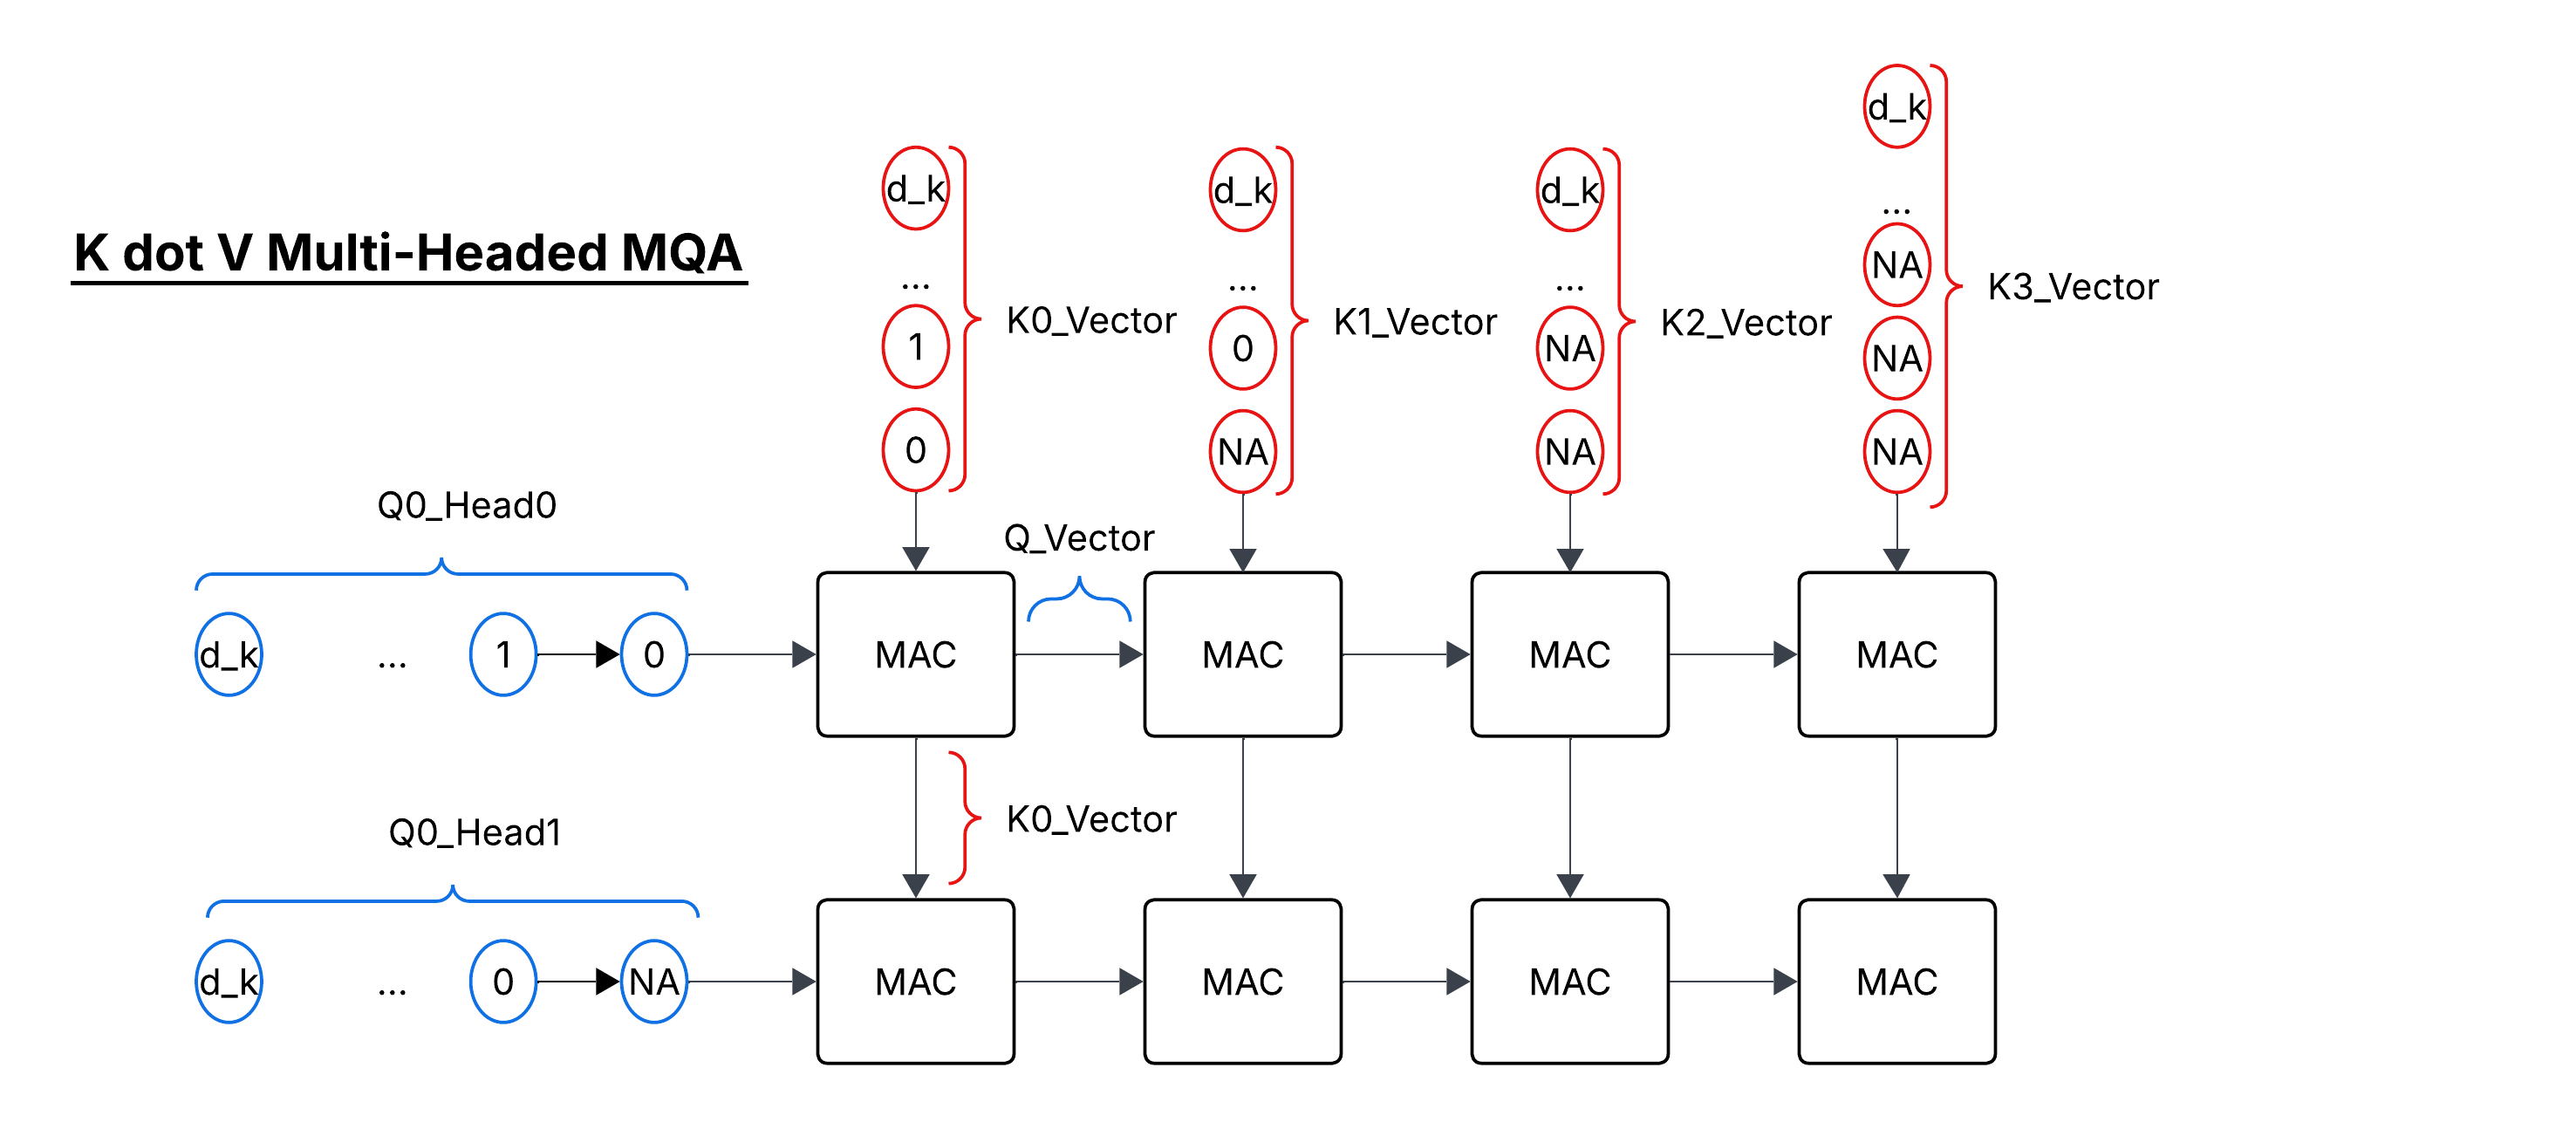
\includegraphics[width=\textwidth]{MultiHeaded.png}
        \caption{Multi-head MQA layout. $H$ row lanes share one set of KV
        columns; KV is loaded from DRAM exactly once regardless of head count.}
    \end{subfigure}\hfill
    \begin{subfigure}[t]{0.49\textwidth}
        \centering
        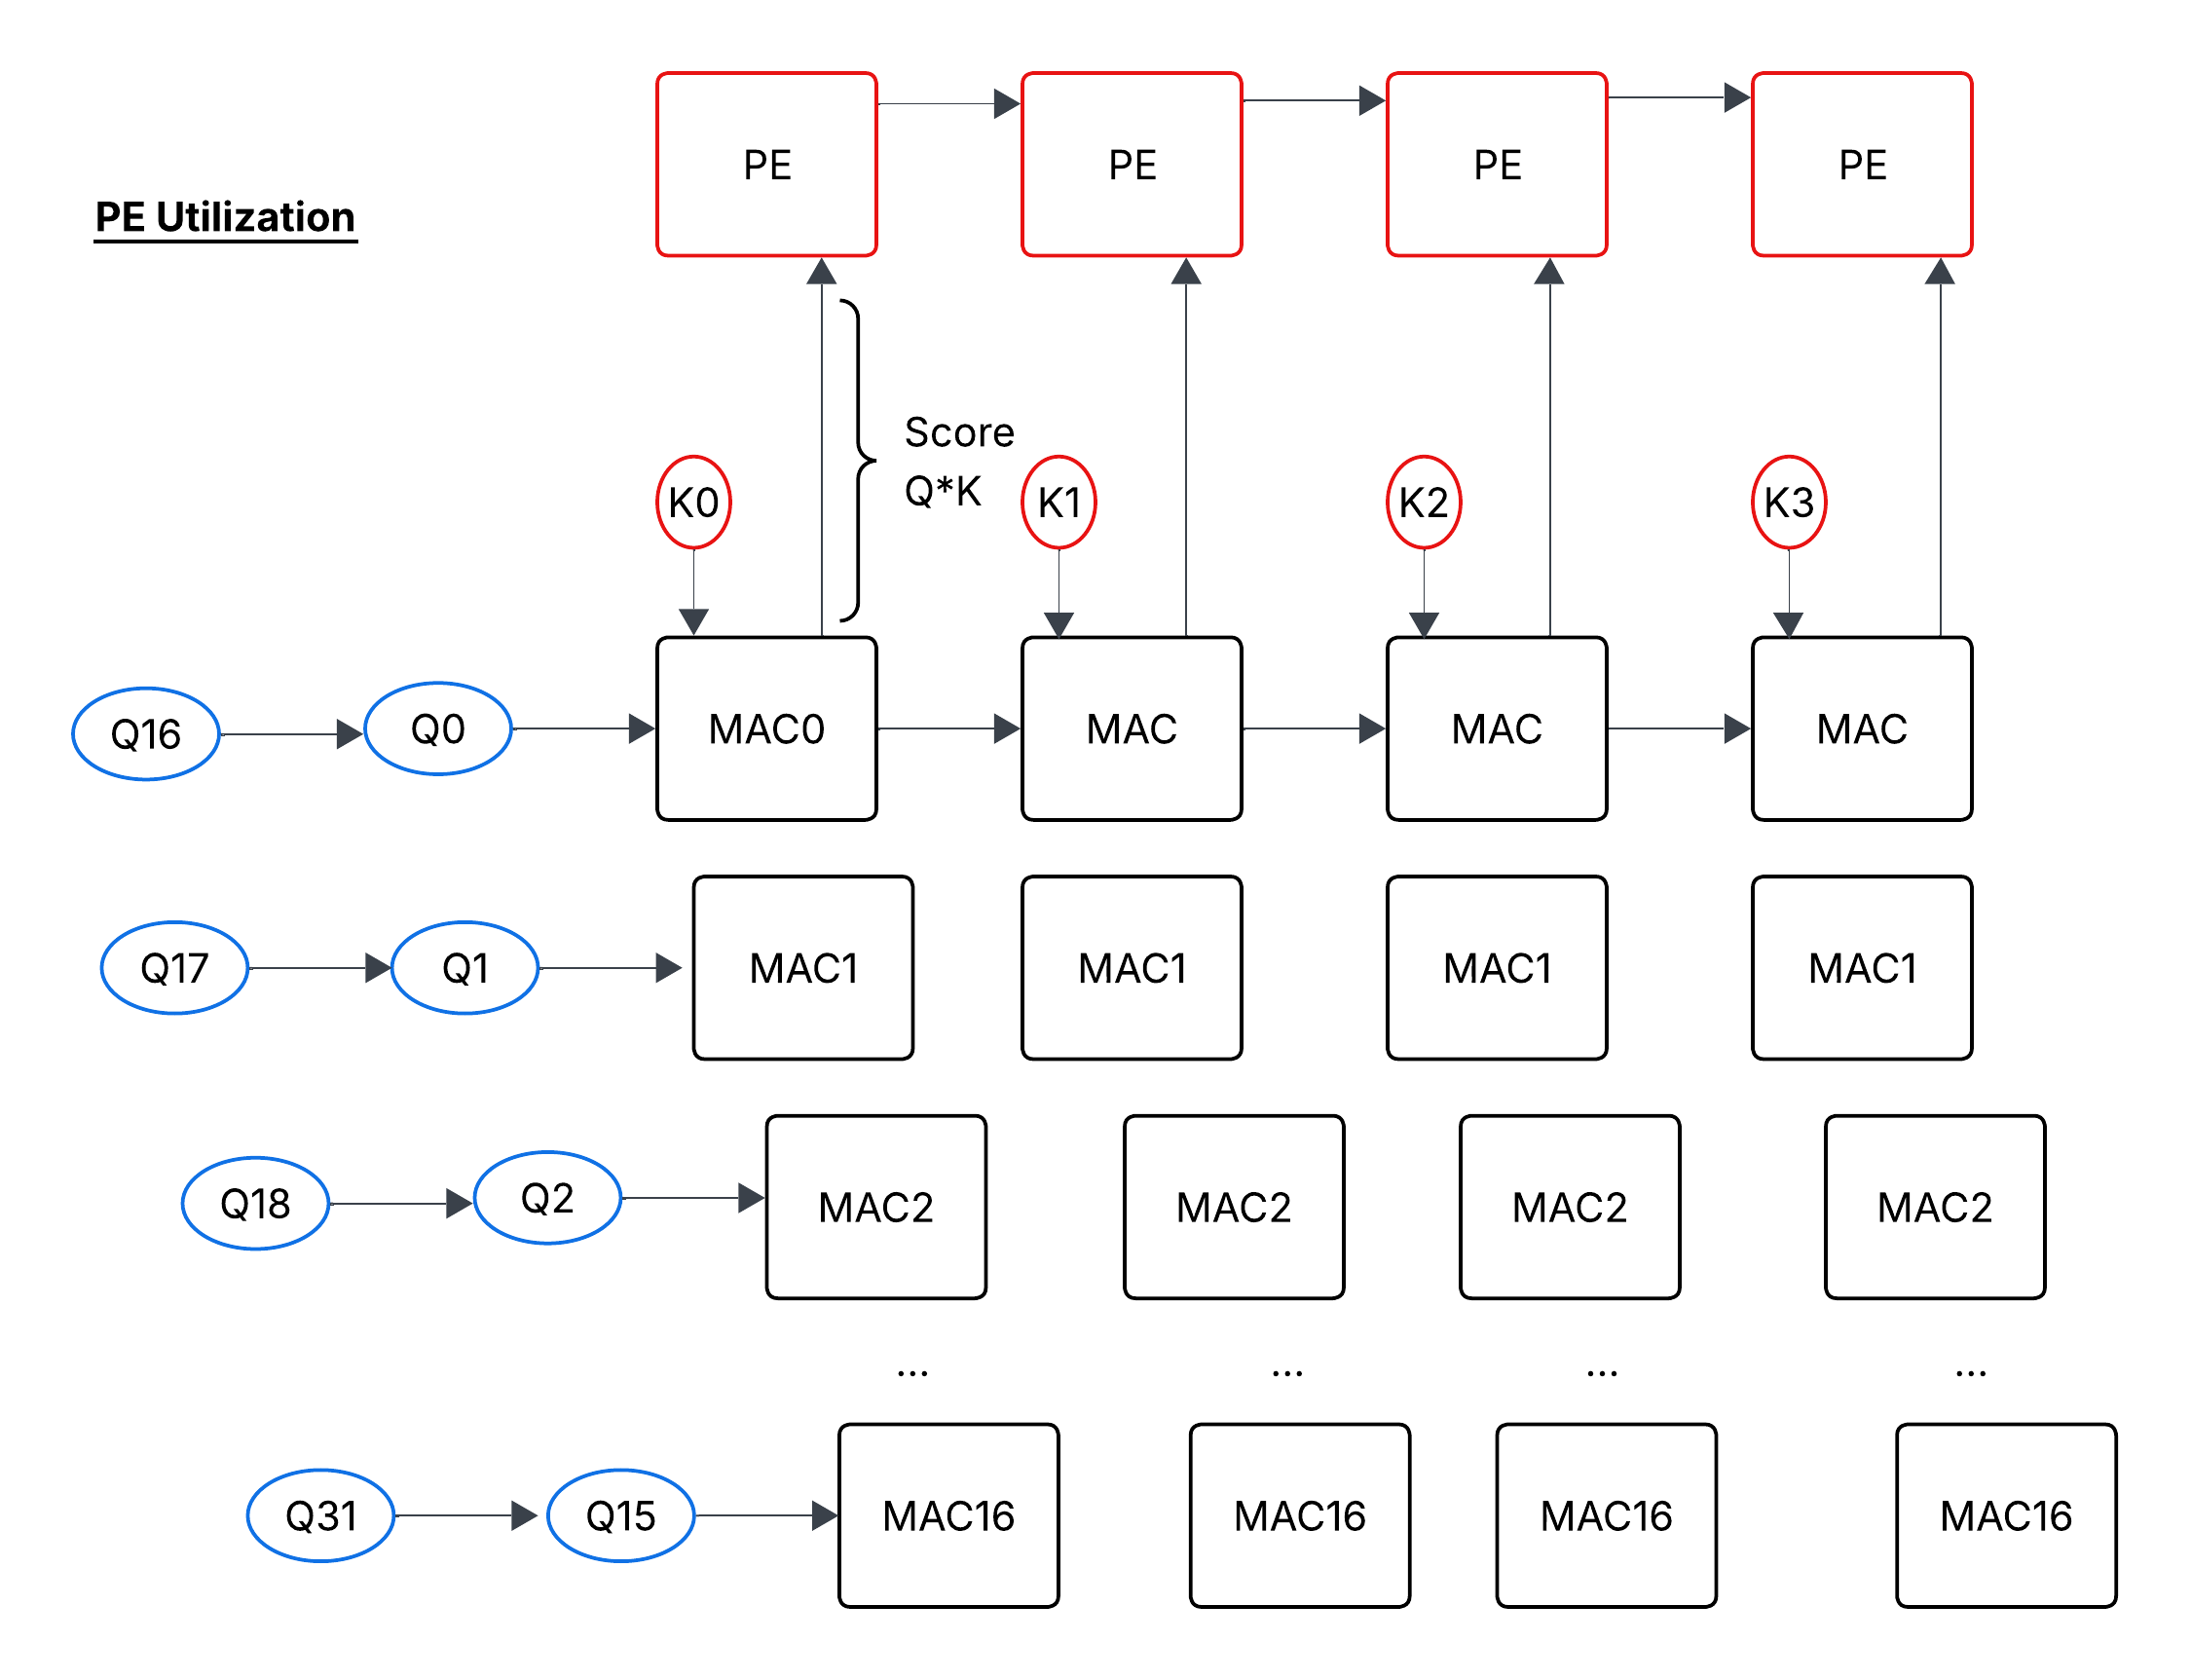
\includegraphics[width=\textwidth]{PEUtilization.png}
        \caption{$lmc{=}16$ time-interleaved MACs. 16 query packets share one
        column staggered by 8 cycles; upper-PE utilization rises to 87.5\%.
        Throughput ceiling: $lmc{=}21$ ($\lceil 128/21\rceil{=}7$ exactly
        matches the 7-cycle upper-PE cost); beyond this the score buffer
        activates but no further throughput is gained.}
    \end{subfigure}
    \caption{KV-stationary array. Queries stream left-to-right; KV is
    stationary; online softmax runs inline, eliminating the $H{\times}T^2$
    score-matrix DRAM round-trip.}
    \label{fig:arch}
\end{figure}

\subsection{Pipeline Timing Model}

Because every column owns a \emph{dedicated} lower MAC and stationary $K_i$, a
packet's $C$ dot products $s_0{\ldots}s_{C-1}$ are independent and compute in a
pipelined wavefront as $Q$ ripples right.
The $d{=}128$ fill is paid \emph{once}; thereafter the binding path is the
online-softmax state chain.
For $R$ active rows, $C$ active columns, $P$ packets per row:
\[
\text{tile\_cycles}
= \underbrace{d}_{\text{fill (once)}}
+ (R + C - 1)\cdot\text{eff\_stagger}
+ (P-1)\cdot\text{eff\_stagger}.
\]
SCALE-Sim measures $\sim\!2.5$ cycles/column of fill, confirming the wavefront model (\S\ref{sec:wavefront}).

\textbf{DRAM traffic.}
At $T{=}8{,}192$: $Q$ reads $+$ $KV$ load $+$ $O$ writes $\approx 273$ MB (FP16),
identical to a fused FlashAttention baseline.
An \emph{unfused} baseline adds the score matrix
($H{\times}T^2{\times}\text{bpe} = 17.18\,\text{GB}$ written then re-read $= 17.18\,\text{GB}$),
bringing total unfused DRAM to 17.45\,GB of which the score matrix is 98.4\%.
Arithmetic intensity (MACs/byte) at $T{=}8{,}192$: unfused baseline 63 (compute-bound);
fused FlashAttention 4,033 (memory-bound); KV-stationary 8,066 (memory-bound,
2$\times$ higher due to the additional $3d$ V-accumulation MACs per token pair).
The identical DRAM traffic of the latter two explains why their cycle counts converge
when both are memory-bound.

\subsection{Implementation}

The model is implemented in Python with five key files:
\texttt{kv\_stationary\_model.py} (analytical pipeline, wavefront fill model, multi-pass re-use extension),
\texttt{baseline\_mqa\_model.py} (roofline baseline, fused/unfused),
\texttt{validate\_lower\_mac\_sweep.py} and \texttt{validate\_sweep\_scalesim.py}
(SCALE-Sim harness),
and \texttt{reuse\_full\_sweep.py} (750-row bandwidth$\times$lmc$\times$T$\times$P
sweep).
SCALE-Sim validates the $Q{\cdot}K$ GEMM at infinite bandwidth to isolate compute;
the analytical model adds a roofline DRAM floor:
\begin{align*}
\text{corrected\_cyc} &= \text{pipeline\_cyc} - \text{analytical\_mac} + \text{ss\_mac\_cyc},\\
\text{total\_cyc} &= \max(\text{corrected\_cyc},\;\text{DRAM\_cyc}).
\end{align*}

% ============================================================
\section{Experimental Results and Evaluation}

\paragraph{Setup.}
Fixed hardware: $H{=}64$, $d{=}128$, FP16 (2 B/elem), DRAM BW $= 512$ B/cycle,
upper-PE width $w{=}128$, $\tau_{\exp}{=}4$ cycles.
Sweep: $T \in \{128,512,1024,2048,4096,8192\}$;
$n \in \{0,3\}$; $lmc \in \{1,2,4,8,16\}$; prefill ($Q_T{=}T$).
SCALE-Sim ran on 40 prefill configurations fitting the 500\,MB operand-matrix
limit; 9 large configurations ($n{=}0$, $lmc{=}16$, $T{\ge}4096$) are
analytical only.
Decode validation failed (analytical diverges thousands of percent from
SCALE-Sim because the model counts only $d$ MAC cycles while SCALE-Sim measures
the full pipeline traversal); decode results are excluded.

\subsection{SCALE-Sim Validation and the Wavefront Fill}
\label{sec:wavefront}

Table~\ref{tab:mac_validation} shows representative results; $\delta\%$ is the
SCALE-Sim excess over the analytical MAC bound --- the pipeline fill physically
observed, \emph{not} a modeling error.
Across all 40 runs, fill clusters at $\sim\!2.5$ cycles/column regardless of
$lmc$, confirming the wavefront fill model.
Under the wavefront fill, prefill is DRAM-bound at every tested configuration.

\begin{table}[H]
\centering
\caption{Lower-MAC SCALE-Sim validation (selected prefill).
$\delta\%$ is the measured wavefront fill as a fraction of the analytical MAC
bound. Errors below 10\% at $T{\ge}1024$ show the model is accurate for large $T$.}
\label{tab:mac_validation}
\small
\begin{tabular}{rrrrrr}
\toprule
$T$ & $n$ & $lmc$ & Analytical & SCALE-Sim & $\delta\%$ \\
\midrule
128  & 0 &  1 & 16,384 & 16,891 &  3.1\% \\
512  & 0 &  1 & 65,536 & 66,811 &  1.9\% \\
512  & 0 & 16 &  4,096 &  5,371 & 31.1\% \\
2048 & 0 & 16 & 16,384 & 20,731 & 26.5\% \\
2048 & 3 & 16 & 16,384 & 17,147 &  4.7\% \\
8192 & 3 & 16 & 65,536 & 67,835 &  3.5\% \\
\bottomrule
\end{tabular}
\end{table}


\subsection{Bandwidth Co-Design: Sizing $lmc$ to Bandwidth}

With the validated wavefront fill, compute at $T{=}8{,}192$ drops to
$\sim\!132$K cycles for $lmc{=}16$ --- far below the DRAM floor of $\sim\!525$K
cycles at 512\,B/cycle.
Compute scales as $1/lmc$ while the DRAM floor is fixed by bandwidth, so they
cross at $lmc \approx \text{BW}/128$ (Figure~\ref{fig:codesign}).
Below this balance point extra MACs sit idle: at $lmc{=}16$ on 512\,B/cycle,
75\% of multipliers are stalled, and per-MAC efficiency is only $0.26\times$.
\emph{This inverts the earlier design recommendation}: $lmc{\le}4$ is the
efficient choice at 512\,B/cycle; $lmc{=}16$ is only justified with
$\sim\!2$\,TB/s (HBM-class) bandwidth, where it runs $4\times$ faster.

\begin{figure}[H]
    \centering
    \begin{subfigure}[t]{0.49\textwidth}
        \centering
        
\includegraphics[width=\textwidth]{fig15_compute_vs_dram_floor.png}
        \caption{Compute ($\propto 1/lmc$) crosses the DRAM floor at
        $lmc{\approx}\text{BW}/128$; past it, MACs idle.}
    \end{subfigure}\hfill
    \begin{subfigure}[t]{0.49\textwidth}
        \centering
        
\includegraphics[width=\textwidth]{fig14_lmc_bw_codesign.png}
        \caption{Per-MAC efficiency vs $lmc$ per bandwidth tier.
        The optimum ($\star$) marches right as bandwidth grows.}
    \end{subfigure}
    \caption{$lmc$--bandwidth co-design at $T{=}8{,}192$. At commodity
    512\,B/cycle the balance point is $lmc{\approx}4$.}
    \label{fig:codesign}
\end{figure}

\subsection{Prefill: KV-stat vs FlashAttention on Equal Silicon}

Table~\ref{tab:prefill_results} compares KV-stat against a fused FlashAttention
baseline running on a single $H{\times}H{=}64{\times}64$ array.
Both eliminate score-matrix DRAM.
\emph{Raw} speedup uses this single-array Flash cycle count directly.
\emph{Per-MAC} $=$ raw speedup $\div$ physical-MAC ratio
($\text{KV\_MACs}/\text{Flash\_MACs}$), which adjusts for the fact that KV-stat
deploys many more multipliers; above $1.0\times$ means KV-stat delivers more
throughput per multiplier.

\begin{table}[H]
\centering
\caption{Prefill: KV-stat vs fused FlashAttention (wavefront model).
DRAM-bound = 512\,B/cycle; Compute-only = no memory wall (SCALE-Sim regime).
$^\dagger$ = analytical (operand-limit exceeded).}
\label{tab:prefill_results}
\small
\begin{tabular}{lr rr rr r}
\toprule
& & \multicolumn{2}{c}{DRAM-bound} & \multicolumn{2}{c}{Compute-only} & \\
\cmidrule(lr){3-4}\cmidrule(lr){5-6}
Config & $T$ & Raw & per-MAC & Raw & per-MAC & MAC ratio \\
\midrule
$n{=}0,\;lmc{=}1$  &  512 &   7.9$\times$ & 1.00$\times$ &   7.9$\times$ & 1.00$\times$ &     8$\times$ \\
$n{=}0,\;lmc{=}1$  & 8192 & 133$\times$   & 1.04$\times$ & 133$\times$   & 1.04$\times$ &   128$\times$ \\
\midrule
$n{=}0,\;lmc{=}16$ &  512 &  33$\times$   & 0.26$\times$ & 124$\times$   & 0.97$\times$ &   128$\times$ \\
$n{=}0,\;lmc{=}16$ & 8192$^\dagger$ & 527$\times$ & 0.26$\times$ & 2133$\times$ & 1.04$\times$ & 2048$\times$ \\
\midrule
$n{=}3,\;lmc{=}16$ & 2048 & 134$\times$   & 0.26$\times$ & 775$\times$   & 1.51$\times$ &   512$\times$ \\
$n{=}3,\;lmc{=}16$ & 8192 & 535$\times$   & 0.26$\times$ & 3604$\times$  & $\mathbf{1.76\times}$ & 2048$\times$ \\
\bottomrule
\end{tabular}
\end{table}

Three findings stand out.
\textbf{(1)} At 512\,B/cycle, $lmc{=}16$ sits at $0.26\times$ per MAC ($75\%$
idle); lean $lmc{=}1$ stays compute-bound at $\sim\!1.0\times$.
\textbf{(2)} Merge extensions ($n{=}3$) are \emph{inert} when DRAM-bound --- they
cut column traversal (a compute term) without touching DRAM, so $n{=}0$ and
$n{=}3$ lock to the same floor.
\textbf{(3)} Compute-only, merge extensions \emph{return}: $n{=}3$, $lmc{=}16$
reaches $\mathbf{1.76\times}$ per MAC at $T{=}8{,}192$, where the taller array's
shorter traversal dominates.
Cycle breakdowns and equal-area speedup curves across all four configurations
in the compute-bound regime are in Appendix~\ref{sec:additional}
(Figures~\ref{fig:cycle_breakdown}--\ref{fig:speedup_raw}).

\subsection{Comparison Against Unfused Baseline}

\begin{table}[H]
\centering
\caption{Two-way speedup: KV-stat ($n{=}3$, $lmc{=}16$) vs unfused baselines,
prefill, 512\,B/cycle. The $511\times$ is a MAC-count artifact; the $65\times$
reflects score-matrix DRAM elimination.}
\label{tab:speedup_3way}
\small
\begin{tabular}{rrr}
\toprule
$T$ & vs $64{\times}64$ unfused & vs MAC-norm unfused \\
\midrule
512   &  31.9$\times$ &  5.0$\times$ \\
2,048 & 127.8$\times$ & 17.0$\times$ \\
8,192 & 511.0$\times$ & 64.9$\times$ \\
\bottomrule
\end{tabular}
\end{table}

The $64{\times}64$ baseline is perpetually compute-bound ($7.8\times$ at
$T{=}8{,}192$), making the $511\times$ a MAC-count artifact.
Equalizing MACs flips it memory-bound, paying 17.45\,GB of score-matrix DRAM
(98.4\% of its traffic); both KV-stat and FlashAttention eliminate this,
explaining the $65\times$ over the MAC-matched unfused baseline.
Against the fused baseline --- equal MACs, equal DRAM --- the ratio collapses to
$\sim\!1\times$, confirming DRAM-bound operation.

\subsection{Physical Cost}

Table~\ref{tab:physical_cost} shows the silicon cost behind the raw speedup numbers.

\begin{table}[H]
\centering
\caption{Physical resource requirements for the best prefill configuration
($n{=}0$, $lmc{=}16$). PE count and SRAM scale linearly with~$T$.}
\label{tab:physical_cost}
\small
\begin{tabular}{lrr}
\toprule
Resource & $T{=}8{,}192$ & $T{=}2{,}048$ \\
\midrule
Total PEs            & 524{,}288  & 131{,}072 \\
Total MACs           & 8{,}388{,}608 & 2{,}097{,}152 \\
On-chip K-buffer SRAM & 128\,MB   & 34\,MB \\
Estimated die area   & $\sim$20\,mm$^2$ & $\sim$5\,mm$^2$ \\
\bottomrule
\end{tabular}
\end{table}

The 128\,MB K-buffer at $T{=}8{,}192$ is prohibitive for edge targets; at the
validated $T{=}2{,}048$ point, 34\,MB SRAM and 131K PEs are tractable but still
$32\times$ more PEs than the $64{\times}64$ FlashAttention reference at equal
cycle count.
PE count and SRAM scale linearly with $T$, motivating the multi-pass silicon
re-use scheme (Appendix~\ref{sec:future}).
An energy estimation using Accelergy with CACTI-based component models was
attempted; preliminary component-level breakdowns suggest the primary saving
comes from eliminating the score-matrix DRAM round-trip (which dominates
unfused-baseline energy), but a validated end-to-end figure was not obtained.

% ============================================================
\section{Conclusions}

\paragraph{What worked.}
Three techniques combine to improve attention throughput.
\emph{(1) KV-stationary dataflow with inline online softmax:} keys and values
remain resident in PE columns while queries stream through, computing the
softmax update $m'{=}\max(m,s_i)$, $l'{=}l\,e^{m-m'}{+}e^{s_i-m'}$,
$O'{=}O\,e^{m-m'}{+}V_i\,e^{s_i-m'}$ at each column.
Scores are consumed immediately and never written to DRAM, eliminating the
$H{\times}T^2$ score matrix and yielding a genuine $65\times$ over any unfused
baseline at $T{=}8{,}192$.
\emph{(2) Interleaved MACs ($lmc$):} time-multiplexing $lmc$ independent MAC
units per column, each staggered by $\lceil d/lmc\rceil$ cycles, raises upper-PE
utilization from 5\% to 87.5\% with no extra rows.
\emph{(3) Merge extensions ($n$):} stacking $2^n$ sub-arrays and combining
partial softmax states via a binary merge tree shortens pipeline drain from
$T{-}1$ to $T/2^n{-}1$ column traversals.
The hybrid SCALE-Sim/analytical methodology confirmed wavefront pipelining
at ${\sim}2.5$ cycles/column and established the regime boundary.

\textbf{Compute-bound results.}
When bandwidth is not the bottleneck --- achieved with HBM-class memory or by
reducing $lmc$ to the balance point --- the full benefit of all three techniques
is realised.
In the compute-only limit (Table~\ref{tab:prefill_results}):
$n{=}3$, $lmc{=}16$ reaches $\mathbf{1.76\times}$ per MAC over FlashAttention at
$T{=}8{,}192$, because the taller, narrower sub-array reduces the pipeline
traversal from $8{,}192$ to $1{,}024$ columns.
$n{=}0$, $lmc{=}16$ reaches $1.04\times$ per MAC --- the flat array offers no
drain savings, so the benefit is marginal.
The $1.76\times$ ceiling represents the maximum per-silicon advantage the
KV-stationary approach can deliver over a fused baseline.

\paragraph{What did not work.}
At commodity 512\,B/cycle, maximizing $lmc$ past the balance point
($lmc{\approx}\text{BW}/128$) leaves $75\%$ of MACs idle; the efficient choice
is $lmc{\le}4$, not $lmc{=}16$.
Decode validation also failed: the analytical model counts $d$ MAC cycles per
step while SCALE-Sim measures the full $T$-column pipeline traversal, producing
divergence of thousands of percent.

\paragraph{Conclusion.}
The headline speedup of $511\times$ over a naive unfused baseline is real but
misleading: $98.4\%$ of that baseline's DRAM is the $H{\times}T^2$ score matrix,
which any fused kernel eliminates.
The honest figure is $\mathbf{65\times}$ --- the gain from moving that matrix
off DRAM entirely by computing online softmax inline.
Against a fused FlashAttention baseline on equal silicon, the advantage collapses
to ${\sim}1\times$ at commodity bandwidth, because both architectures are pinned
to the same 273\,MB DRAM floor.

The deeper constraint is \emph{silicon cost}: the array requires one column of
PEs per KV token, so PE count and on-chip SRAM both grow \textbf{linearly with
$T$}.
At $T{=}8{,}192$ that is 524K PEs and 128\,MB of SRAM --- roughly 20\,mm$^2$ of
die area --- with no tested configuration exceeding a $2\times$ area-normalised
advantage.
Scaling context length by $2\times$ doubles the chip.

The multi-pass re-use scheme (Appendix~\ref{sec:future}) breaks this coupling.
Running $P$ passes over $T/P$ physical columns reuses the same array $P$ times,
delivering $P\times$ smaller chip and $P^2\times$ better area-normalised
throughput.
Crucially, the latency cost is sub-linear: at $T{=}8{,}192$ and $P{=}4$ the
pipeline adds only $+2.3\%$ more cycles than a chip $4\times$ larger, because
pipeline drain already dominates at large $T$.
The practical consequence is that validated $T{=}2{,}048$ silicon --- 64 rows,
2{,}048 columns, 32\,MB SRAM --- can serve $T{=}8{,}192$ inference in four
passes at effectively the same latency.

% ============================================================
\section{Team Contributions and Acknowledgement}

\subsection*{Task Allocation}

\begin{center}
\small
\begin{tabular}{ll}
\toprule
Component & Completed by \\
\midrule
Architecture conception \& design iteration & Hudson \\
Analytical pipeline model (\texttt{kv\_stationary\_model.py}) & Hudson \\
Baseline roofline model (\texttt{baseline\_mqa\_model.py}) & Dhruv \\
SCALE-Sim validation harness & Dhruv \\
Architecture diagrams \& visualizations & Hudson \\
Wavefront fill analysis \& BW co-design & Dhruv \\
Sweep scripts \& result CSV generation & Hudson \\
Figure-plotting scripts & Dhruv \\
DRAM traffic analysis \& energy estimation & Hudson \\
Report writing \& editing & Both \\
\bottomrule
\end{tabular}
\end{center}

\subsection*{Contributions}

\textbf{Hudson Strauss --- $\sim\!50\%$.}
Led analytical model development, SCALE-Sim validation pipeline, wavefront fill
discovery, bandwidth co-design analysis, and primary report structure.

\textbf{Dhruv Patel --- $\sim\!50\%$.}
Led baseline model implementation, architecture diagrams, DRAM traffic and energy
analysis, result figure generation, and report review.

\clearpage

{\centering\Large\textbf{References, Future Work \& Appendix}\par}
\vspace{1.5em}

\section*{References}

\printbibliography[heading=none]

% ============================================================
\appendix

\section{Future Work: Silicon Re-Use and Two-Pass Decode}
\label{sec:future}

The primary barrier to practical decode deployment is on-chip SRAM.
At $T{=}8{,}192$ the full KV cache requires 128\,MB --- prohibitive for edge
or embedded targets.
A \textbf{multi-pass silicon re-use scheme} addresses this directly.

\paragraph{Concept.}
Rather than holding the entire KV cache on-chip across all tokens, the sequence
is partitioned into $P$ equal slices of $T/P$ tokens each.
Each decode step makes $P$ passes over the same physical array (now sized
$H \times T/P$ columns), accumulating the running softmax state $(m, l, O)$
across passes using the same online-softmax merge formula used by the merge tree
for prefill.
After all $P$ passes the final output is produced identically to the single-pass
case.

\paragraph{Hardware cost.}
The array itself is unchanged.
At each pass boundary, the partial state $(m, l, O)$ for each active head ---
$(d+2)$ elements $= 260$ bytes at FP16 --- is written to a small register and
re-injected via a single merge PE (Figure~\ref{fig:merge_unit}) at the start of the next pass.
This re-injection costs $2\tau_{\exp} + \lceil 6d/w \rceil = 8{+}6 = 14$ cycles
per pass boundary, negligible relative to single-pass cycles (${\sim}1$M at
$T{=}8{,}192$).

\begin{figure}[H]
    \centering
    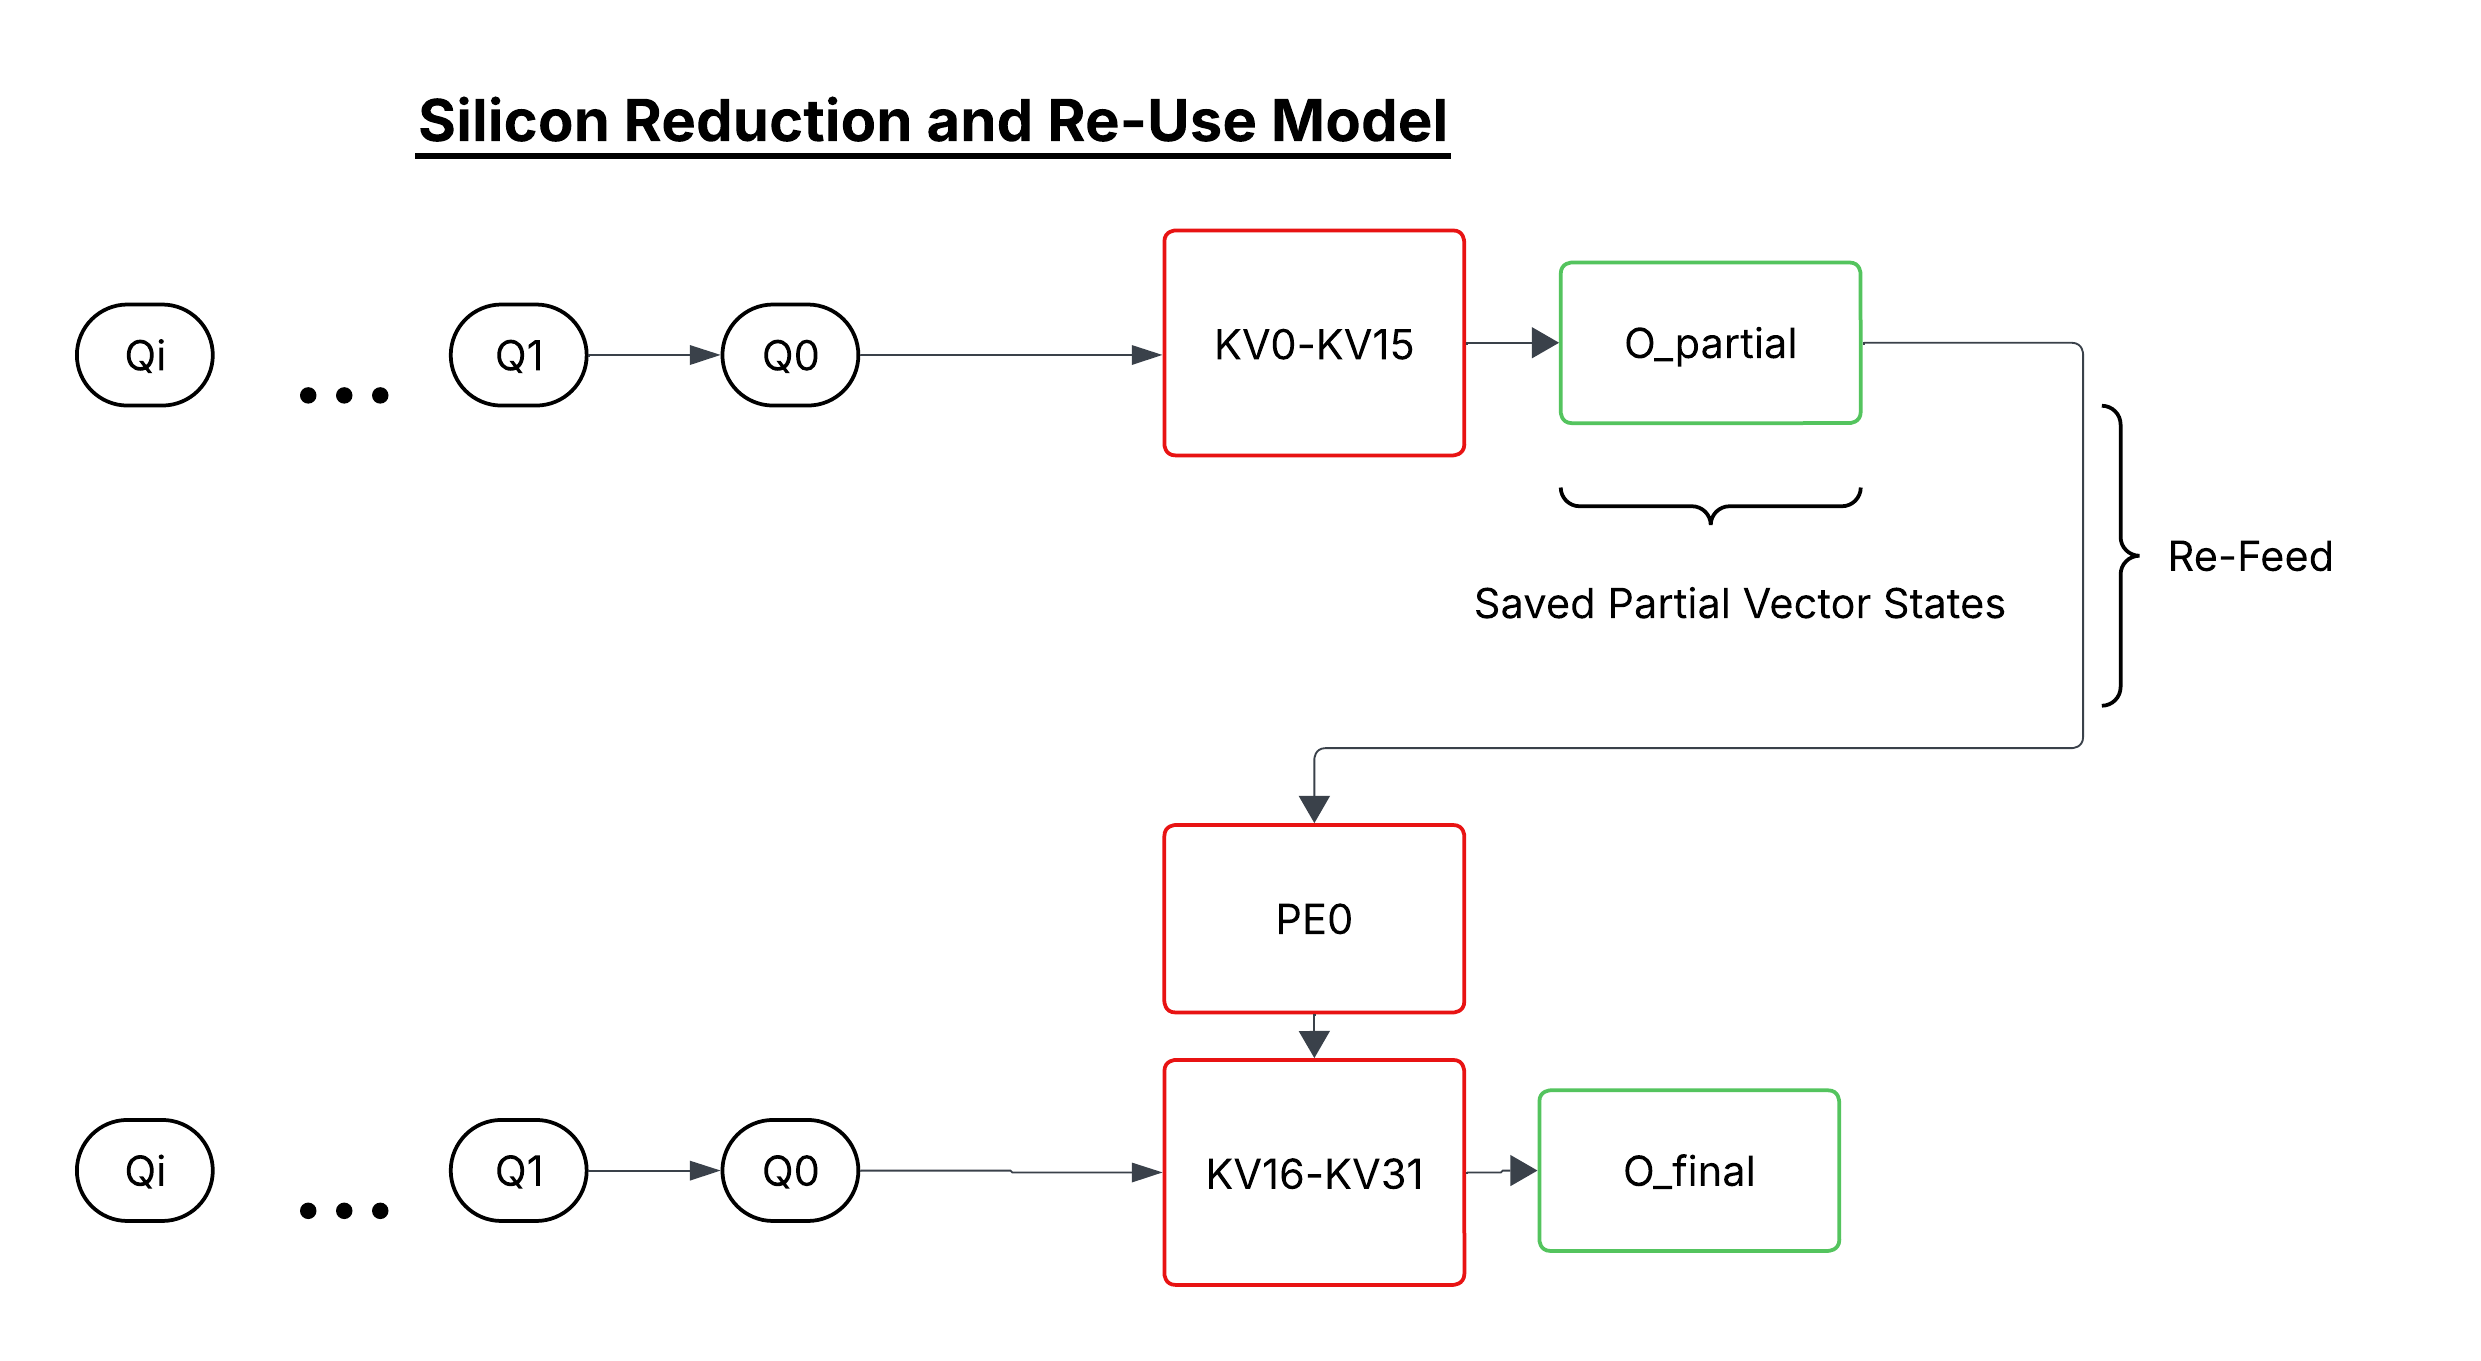
\includegraphics[width=0.82\textwidth]{ReuseModel.png}
    \caption{\textbf{Silicon re-use model ($P{=}2$ passes).}
    Pass~1: the query stream attends over the first KV slice, producing partial
    state \texttt{O\_partial} that is saved.
    Pass~2: the same query re-enters the second slice; the saved state is
    re-injected so the online softmax continues from the correct running maximum.
    \texttt{O\_final} is the correctly normalised output over all $T$ tokens.
    The array uses half the columns (and half the SRAM) of a single-pass design.}
    \label{fig:reuse_model}
\end{figure}

\paragraph{Silicon reduction and the latency trade-off.}

\begin{center}
\small
\begin{tabular}{lrrrr}
\toprule
Passes $P$ & Array cols & On-chip SRAM & Cycle multiplier & Applies to \\
\midrule
1 & $T$     & 128\,MB & $1\times$              & prefill + decode \\
2 & $T/2$   &  64\,MB & ${\approx}2\times$ + 14 cyc & prefill + decode \\
4 & $T/4$   &  32\,MB & ${\approx}4\times$ + 42 cyc & prefill + decode \\
8 & $T/8$   &  16\,MB & ${\approx}8\times$ + 98 cyc & prefill + decode \\
\bottomrule
\end{tabular}
\end{center}

The latency overhead is sub-linear in $P$ at large $T$: the $P{=}1$ pipeline at
$T{=}8{,}192$ is already 99\% drain, so splitting into $P$ smaller passes costs
only $1.02$--$1.11\times$ more total cycles while delivering $P\times$ smaller
chip and $P\times$ less SRAM.
With $P{=}4$ the $T{=}8{,}192$ problem maps exactly to the validated $T{=}2{,}048$
operating point (64$\times$2048 array), running in ${\approx}4\times$ more cycles
with $4\times$ less silicon.
For causal prefill, the savings are even larger: finished queries are discarded at
each pass boundary, reducing Q-read DRAM by up to 69\% at $P{=}16$
(from the 750-row sweep in \texttt{reuse\_full\_sweep.csv}).

\paragraph{Open questions.}
(1) SCALE-Sim cycle validation of a single-pass decode step.
With $\text{query\_tokens}{=}1$ the analytical model counts only $d{=}128$ MAC cycles,
but SCALE-Sim measures the full pipeline traversal: a single Q packet must ripple
through all $T$ columns and drain out, costing ${\approx}(R{+}C{-}1){\times}2$
cycles (${\approx}16{,}500$ cycles at $T{=}8{,}192$, error ${\approx}130{\times}$).
Fixing this requires a traversal-time model rather than a MAC-count model for decode.
(2) Extending the analytical model to multi-pass decode with full inter-pass
softmax merge cost.
(3) Optimal $P$ balancing SRAM budget against acceptable decode latency for the
target workload.

% ============================================================
\section{Architecture Diagrams}
\label{sec:arch_diagrams}

\begin{figure}[H]
    \centering
    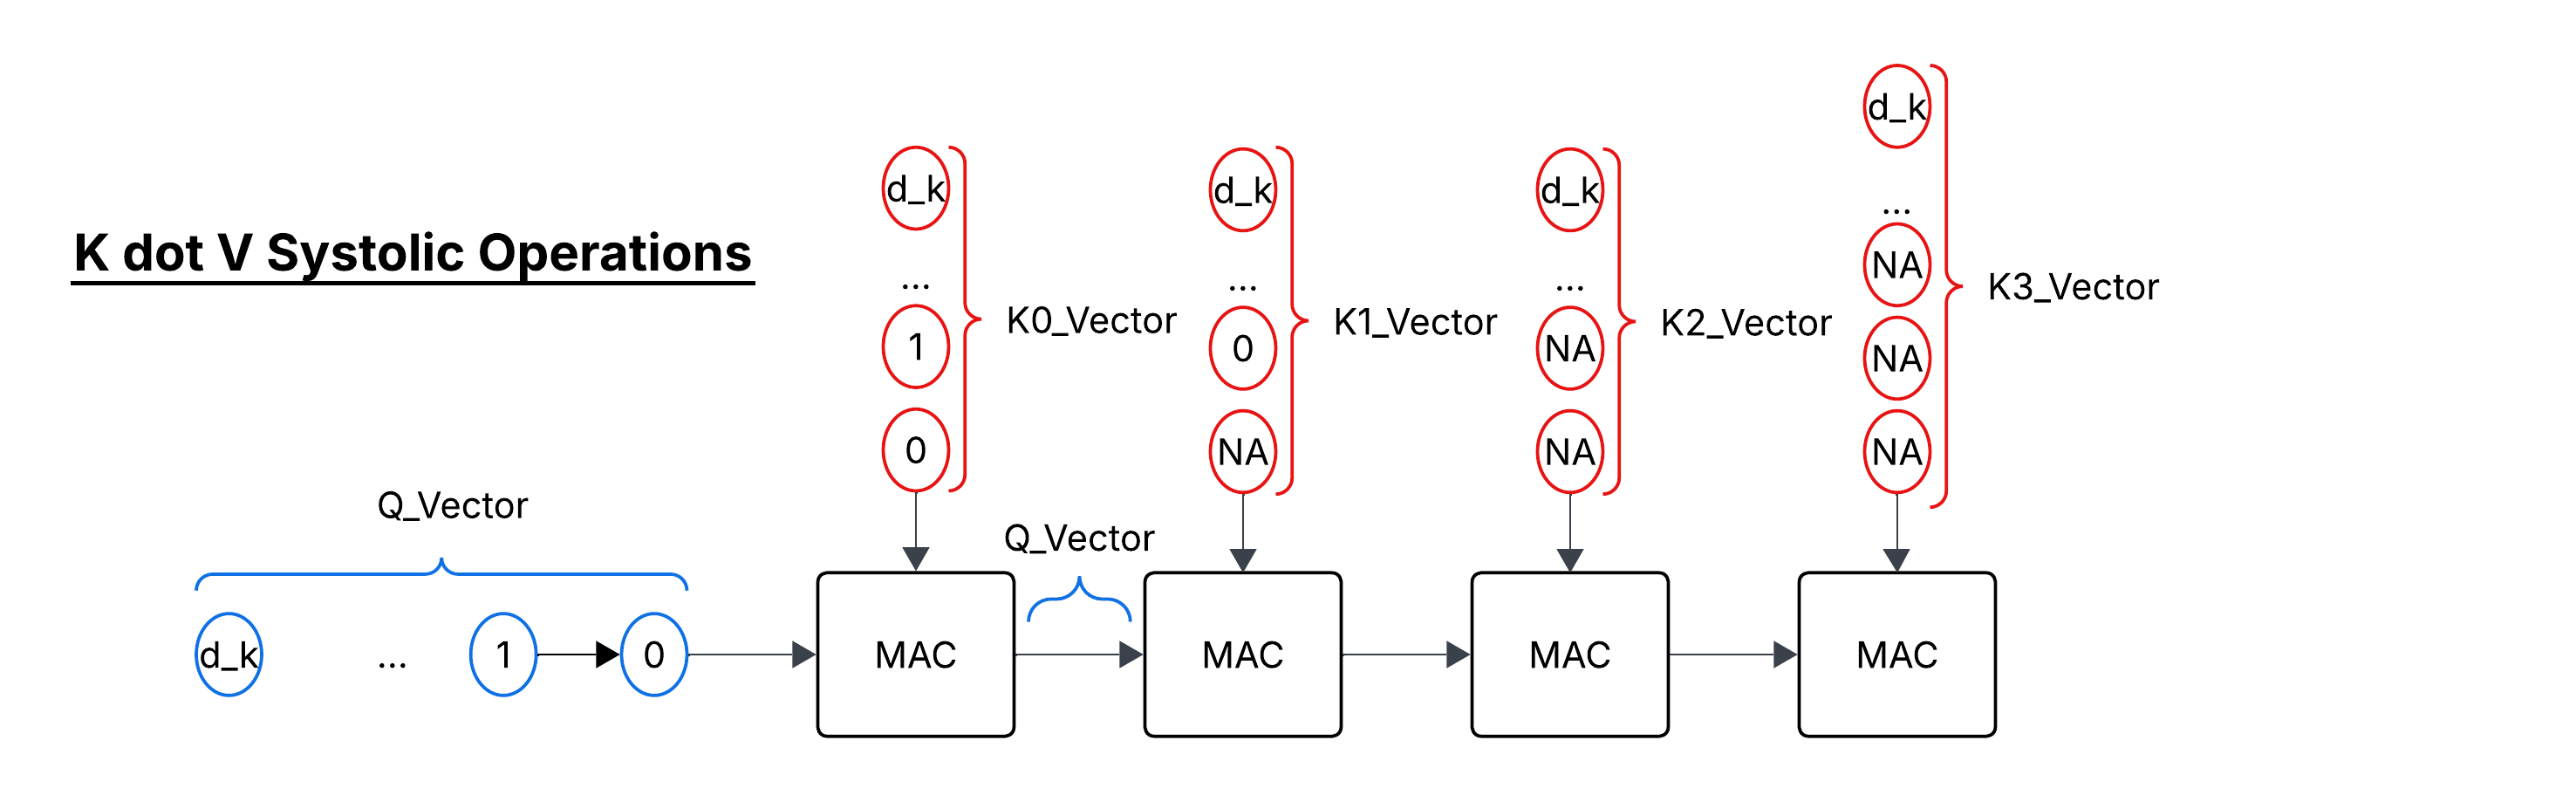
\includegraphics[width=0.72\textwidth]{SystolicSingle.png}
    \caption{Single-row 1D KV-stationary baseline (Iteration~1).
    One query vector $Q$ streams left-to-right through $T$ columns;
    each column holds a stationary $(K_i, V_i)$ pair.
    This is the starting point before multi-head extension, merge extensions,
    and interleaved MACs were added.}
    \label{fig:systolic_single}
\end{figure}

\begin{figure}[H]
    \centering
    \begin{subfigure}[t]{0.48\textwidth}
        \centering
        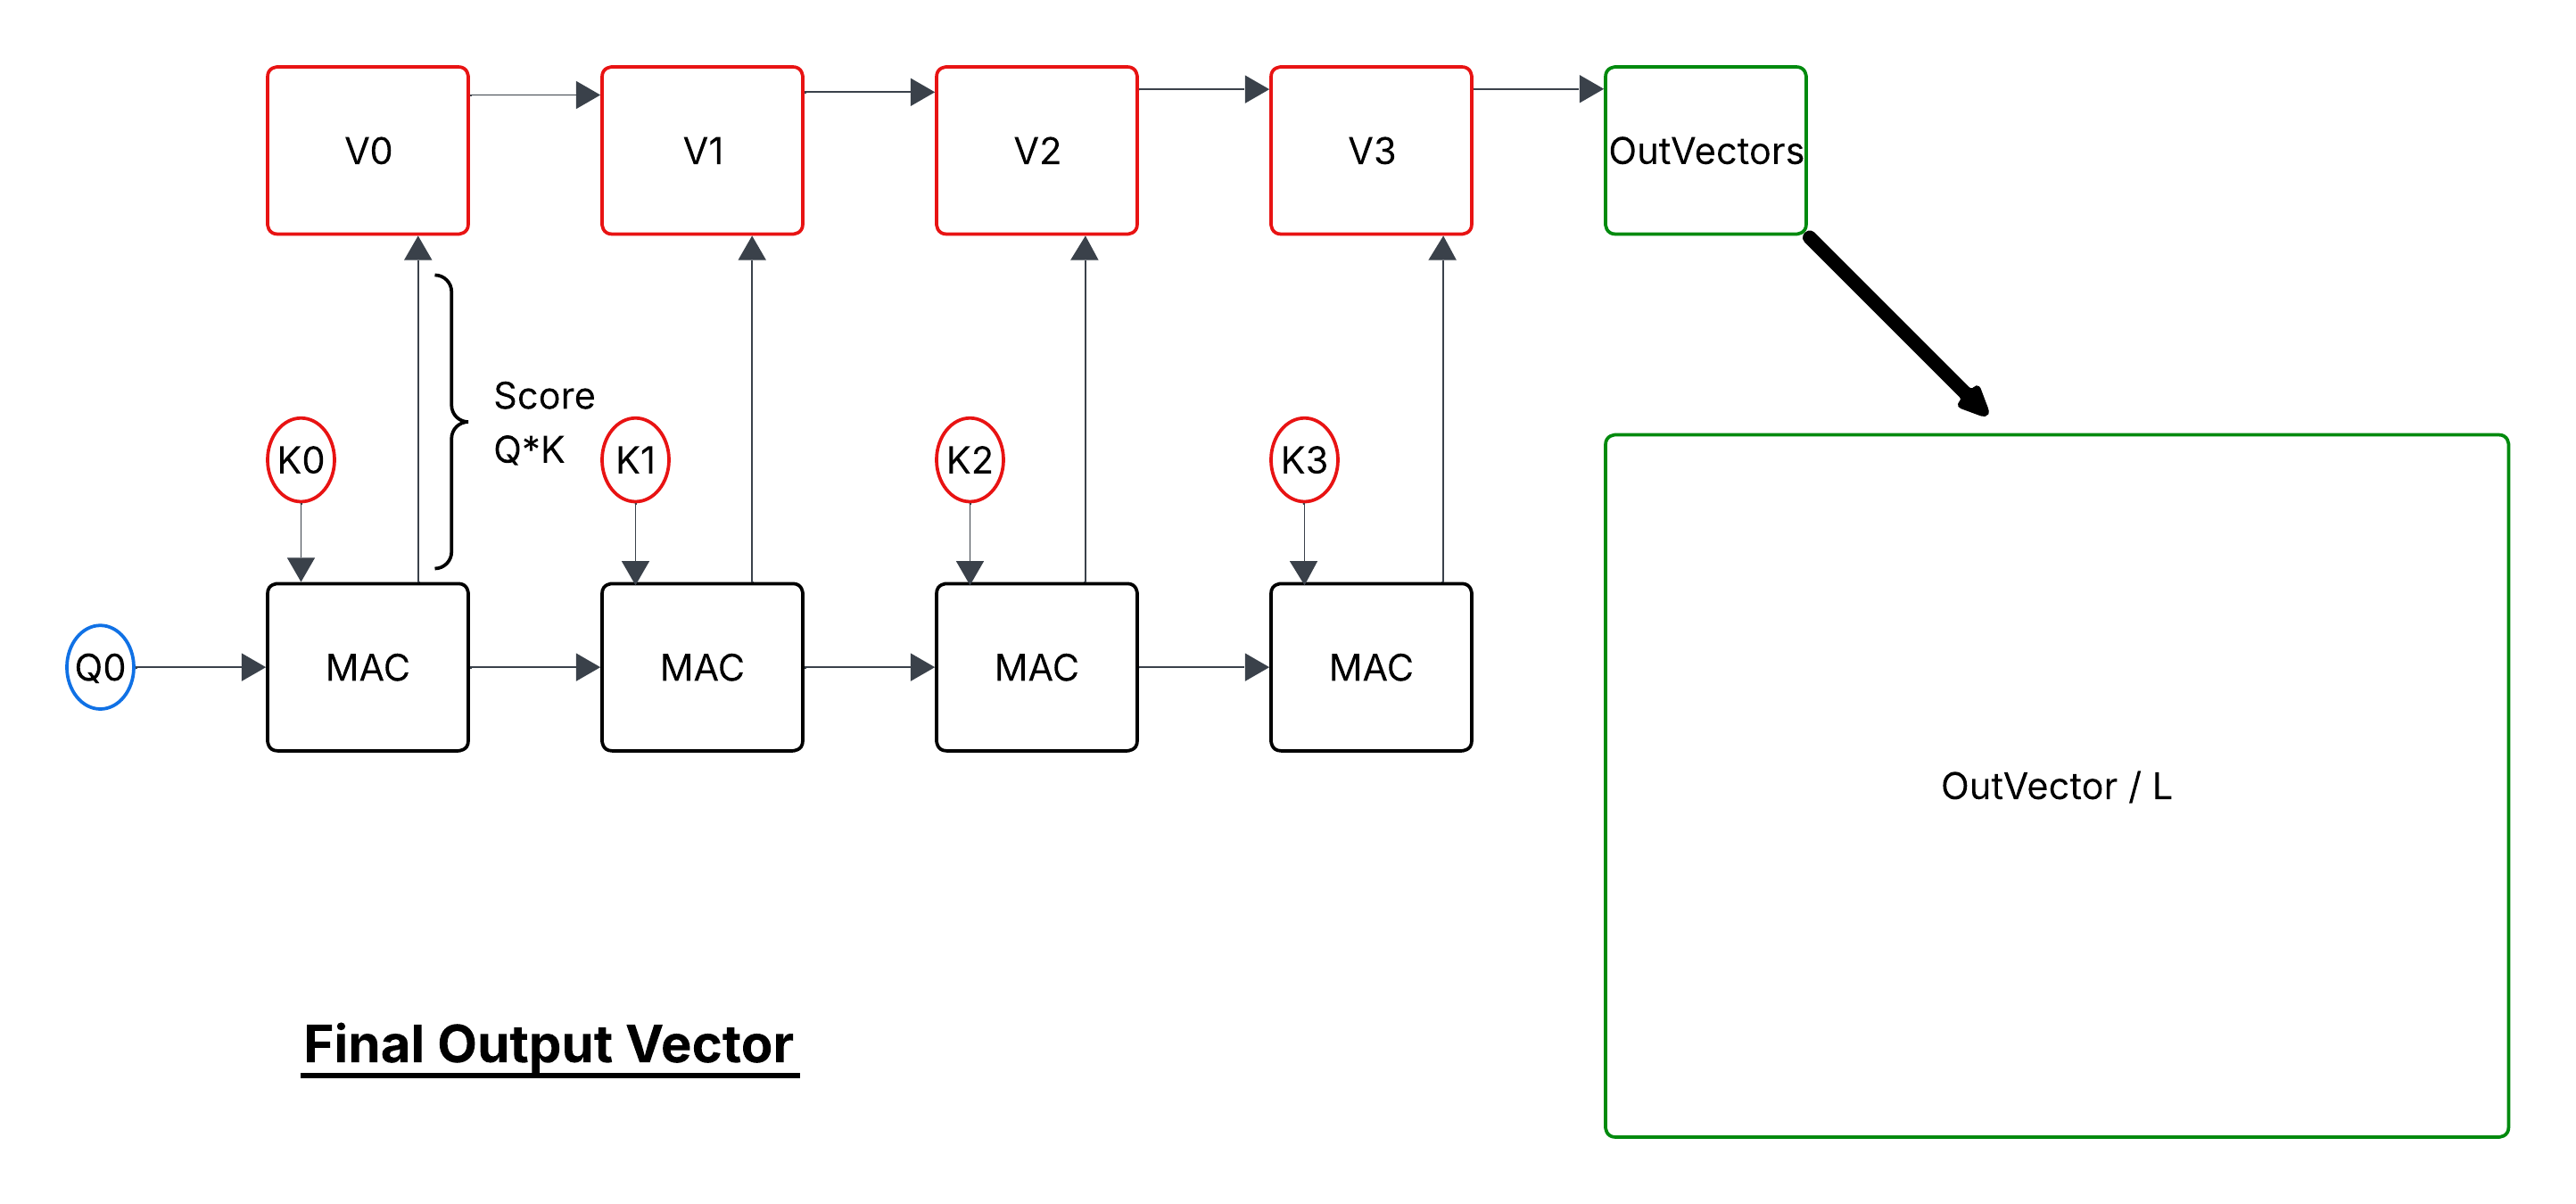
\includegraphics[width=\textwidth]{FinalOutVector.png}
        \caption{Single-row dataflow. Query $Q_0$ streams left-to-right through
        MAC columns; each column computes score $s_i = Q_0 \cdot K_i$ and feeds
        the stationary $V_i$ register above.
        After the final column, \texttt{OutVectors} accumulates the weighted sum
        and normalises by $l_N$ to produce \texttt{OutVector\,/\,L}.}
        \label{fig:final_out_vector}
    \end{subfigure}\hfill
    \begin{subfigure}[t]{0.48\textwidth}
        \centering
        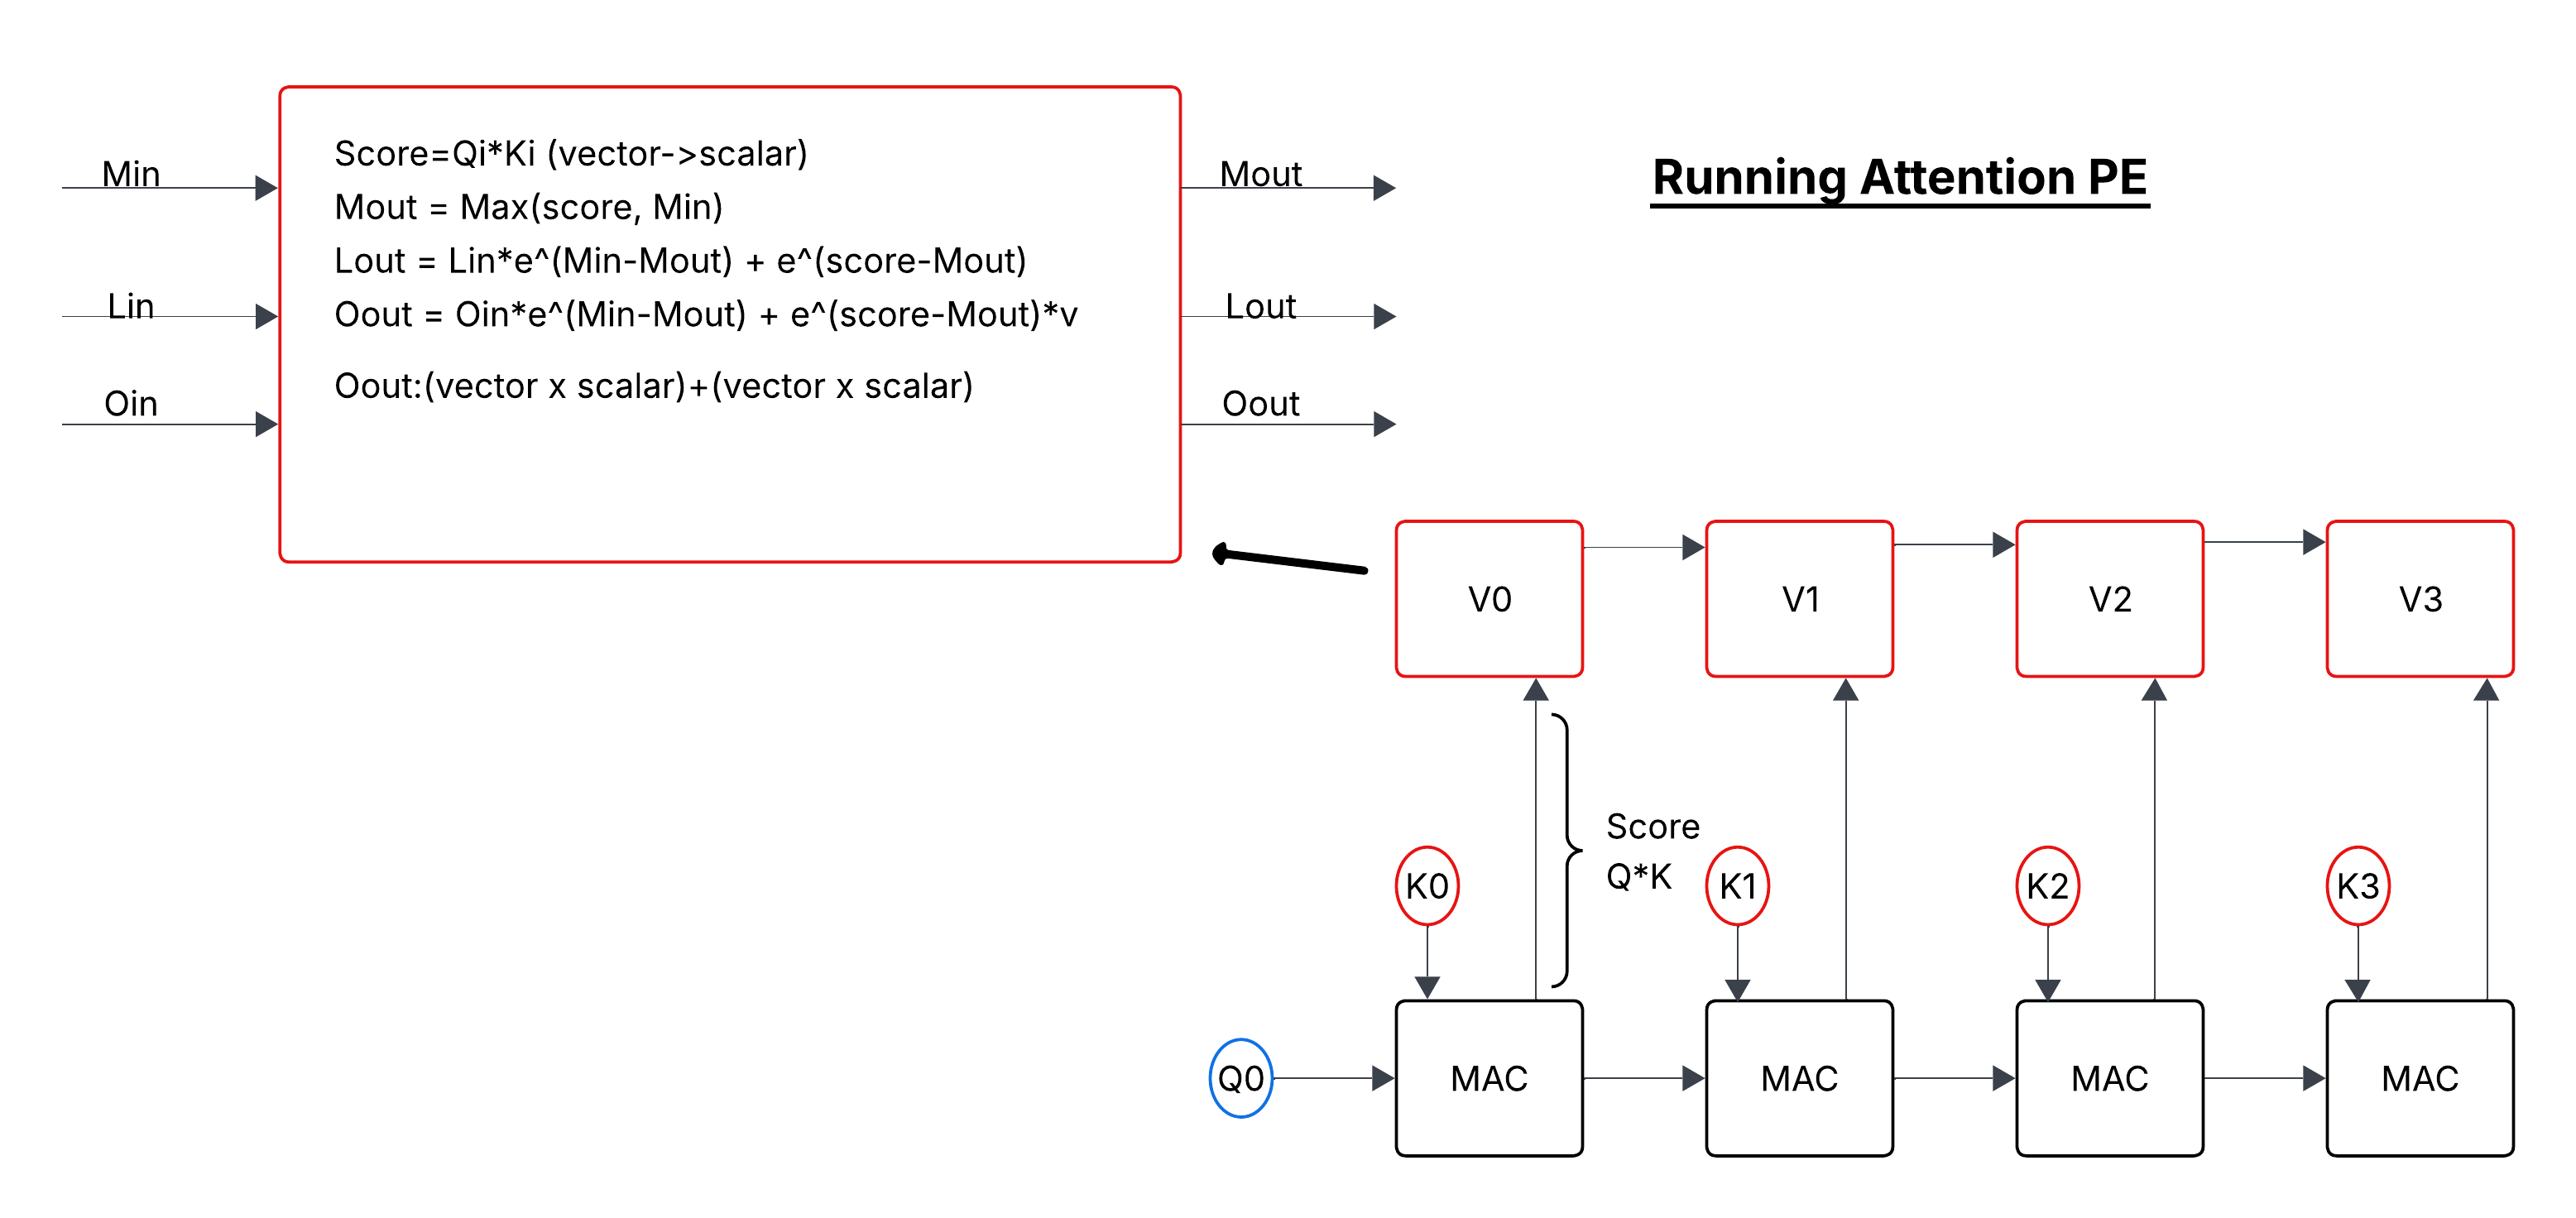
\includegraphics[width=\textwidth]{AttentionPE.png}
        \caption{Running Attention PE detail.
        The PE receives running state $(M_\text{in}, L_\text{in}, O_\text{in})$
        and score $s_i = Q_i \cdot K_i$ (computed below by the MAC array), then
        updates: $M_\text{out}{=}\max(M_\text{in}, s_i)$;
        $L_\text{out}{=}L_\text{in}\,e^{M_\text{in}-M_\text{out}}
        + e^{s_i - M_\text{out}}$;
        $O_\text{out}{=}O_\text{in}\,e^{M_\text{in}-M_\text{out}}
        + e^{s_i - M_\text{out}}{\cdot}V_i$.
        Updated state $(M_\text{out}, L_\text{out}, O_\text{out})$ passes right.}
        \label{fig:attention_pe}
    \end{subfigure}

    \caption{KV-stationary dataflow (left) and Running Attention PE internals
    (right). Together these show how one query head streams through $T$ columns,
    accumulating online softmax state without materialising any score matrix.}
    \label{fig:arch_diagrams}
\end{figure}

\begin{figure}[H]
    \centering
    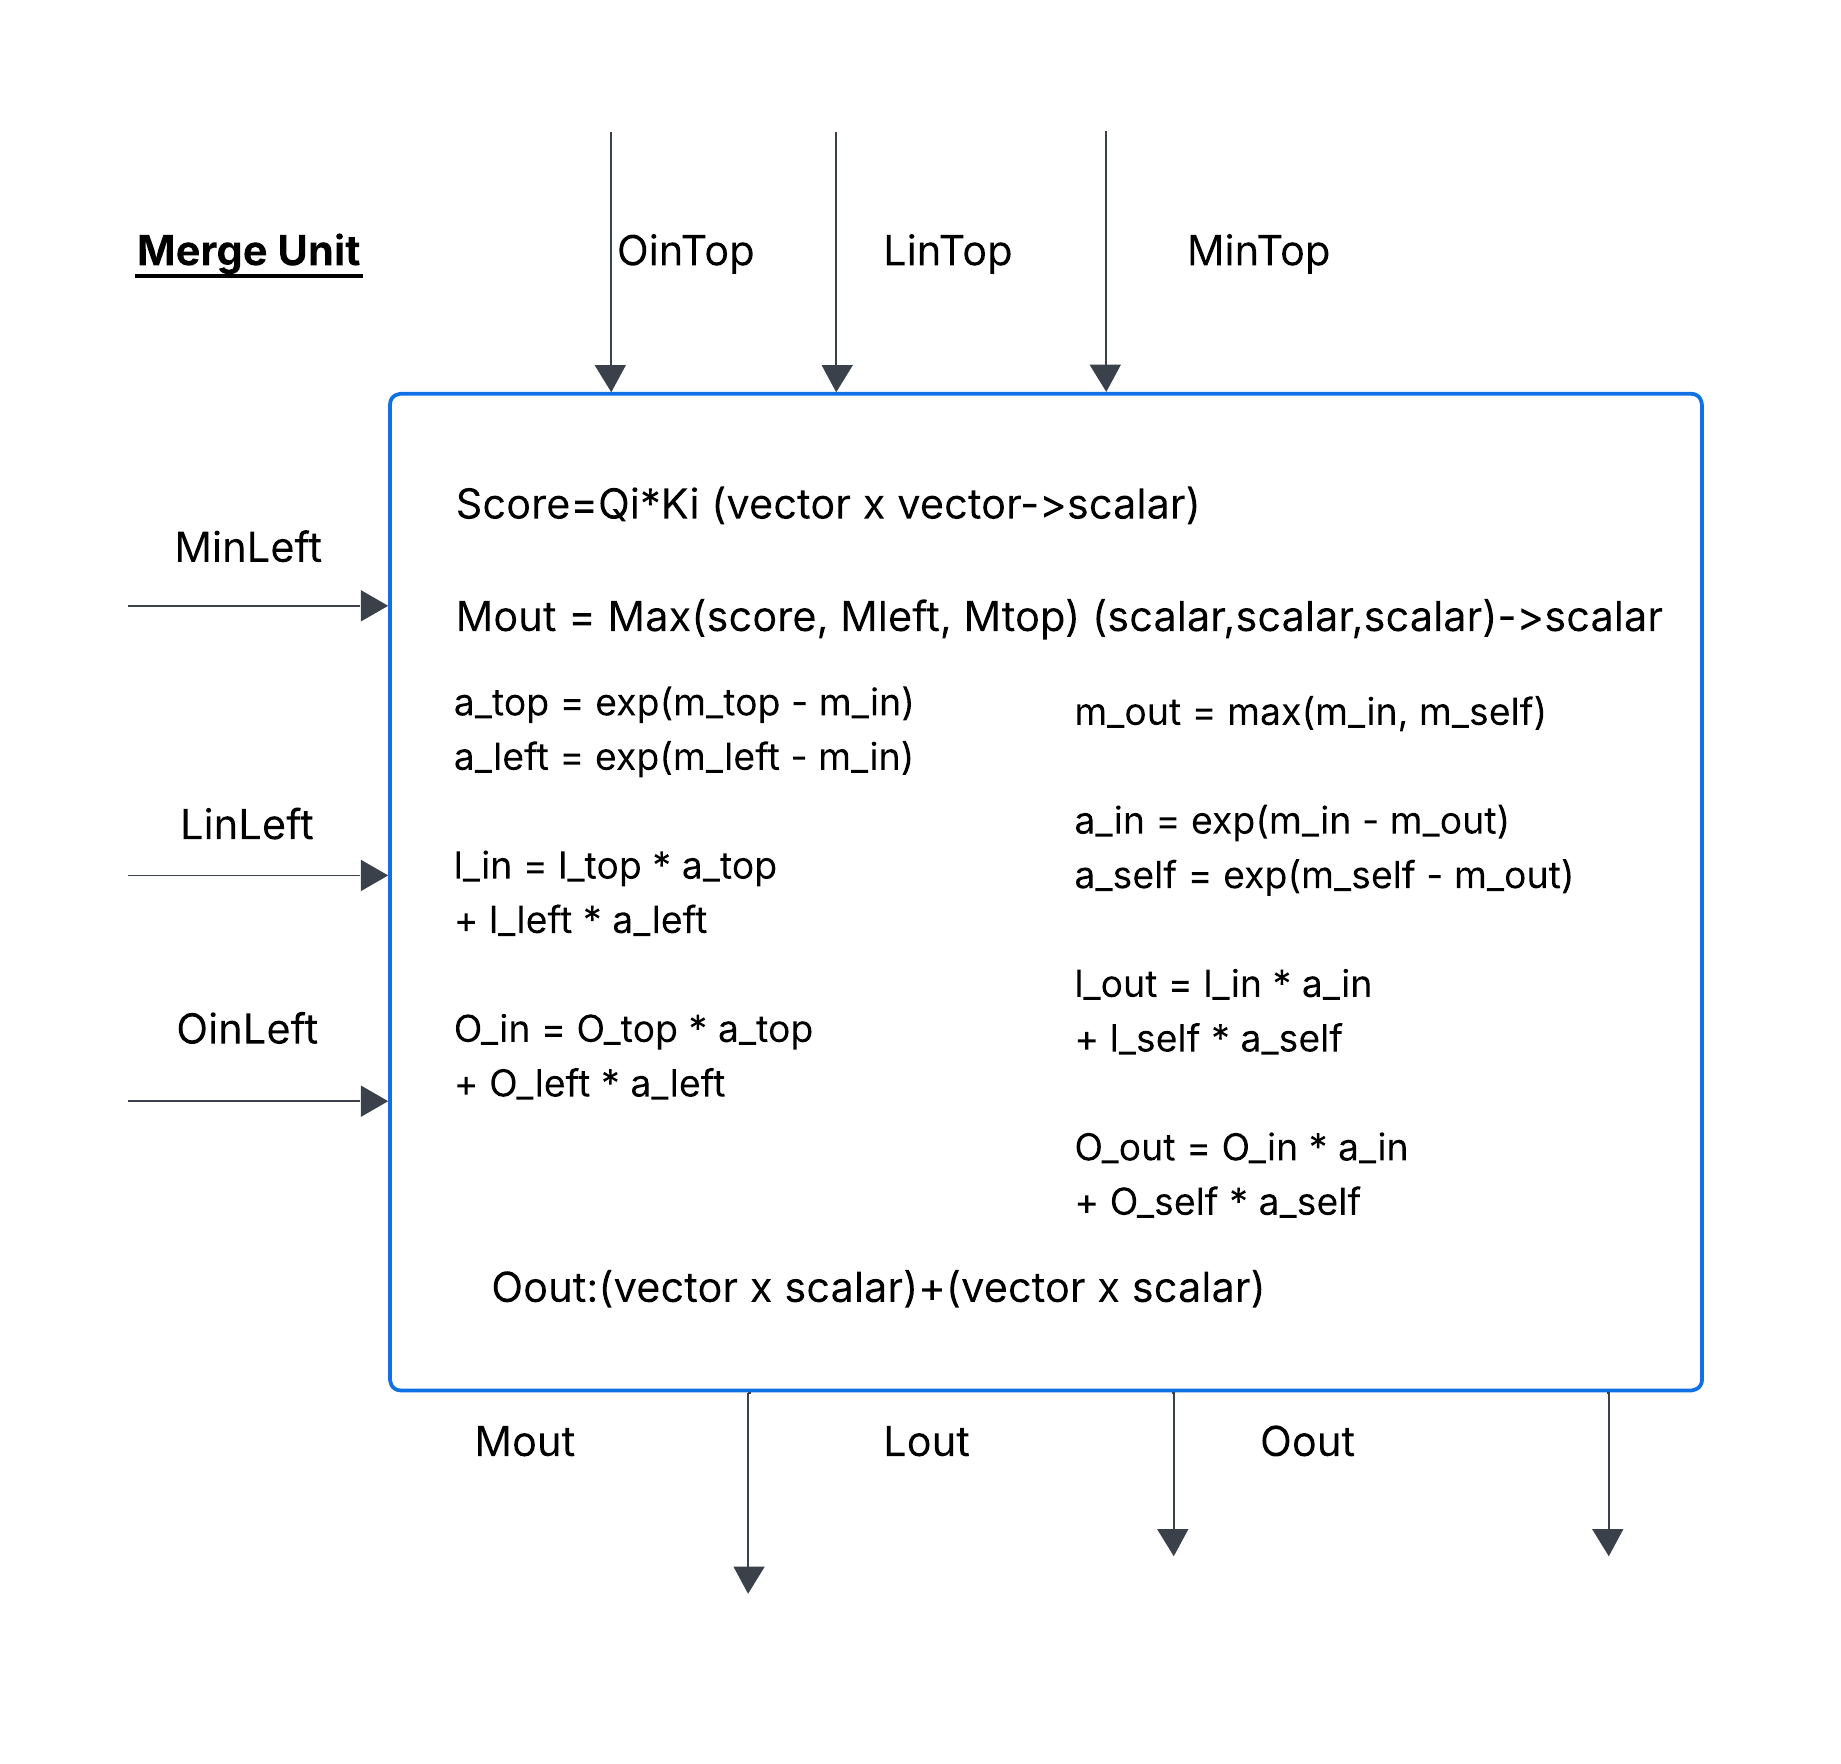
\includegraphics[width=0.72\textwidth]{Merge_unit.png}
    \caption{Merge Unit internals. Receives partial softmax states
    $(M_\text{left}, L_\text{left}, O_\text{left})$ from the row accumulation so far
    and $(M_\text{top}, L_\text{top}, O_\text{top})$ from the top sub-array (or
    previous re-use pass).
    The unit also computes the current-token score $s_i{=}Q_i{\cdot}K_i$, making it
    a combined attention-and-merge PE: $M_\text{out}{=}\max(s_i, M_\text{left}, M_\text{top})$;
    $L_\text{out}{=}L_\text{top}\,e^{M_\text{top}-M_\text{out}}
    + L_\text{left}\,e^{M_\text{left}-M_\text{out}}$;
    $O_\text{out}{=}O_\text{top}\,e^{M_\text{top}-M_\text{out}}
    + O_\text{left}\,e^{M_\text{left}-M_\text{out}}$.
    Note: when used purely for cross-sub-array merging (no new token), $s_i$ is
    omitted and the unit reduces to a two-way state combiner.
    Cost: $2\tau_{\exp} + \lceil 6d/w \rceil = 14$ cycles.}
    \label{fig:merge_unit}
\end{figure}

\begin{figure}[H]
    \centering
    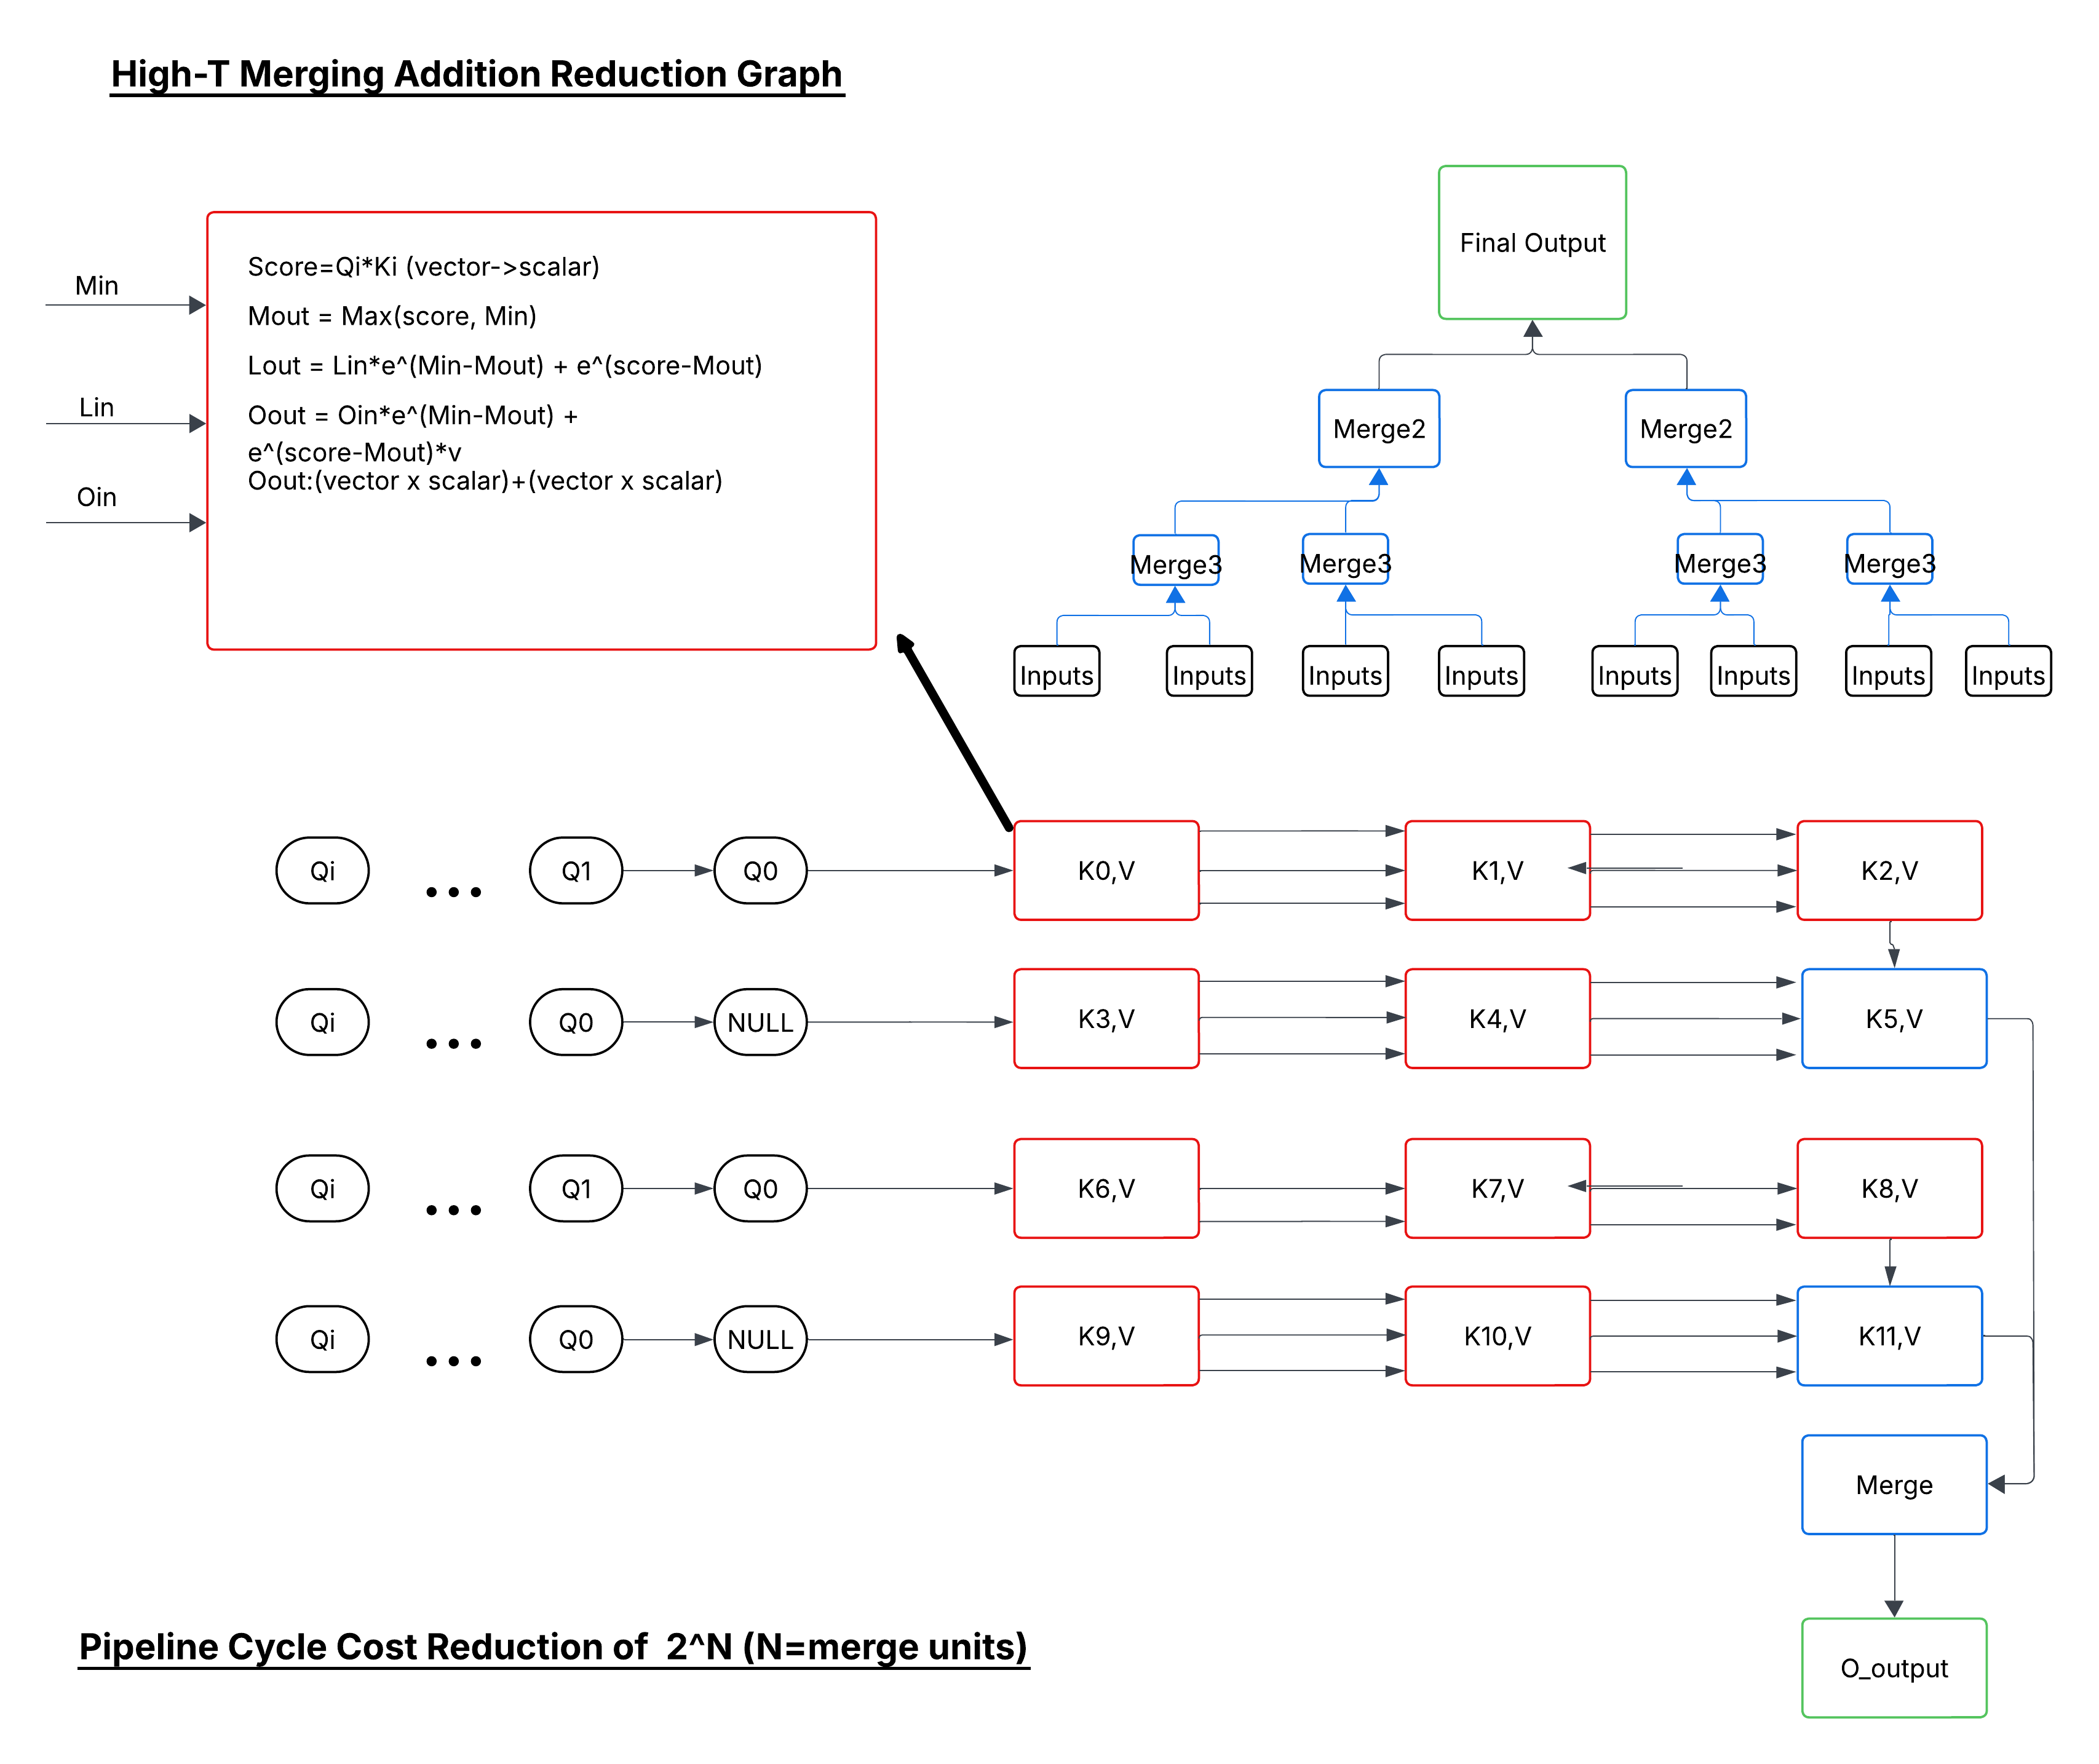
\includegraphics[width=0.72\textwidth]{MergeReductionGraph.png}
    \caption{Merge-extension binary reduction tree ($n{=}3$, eight sub-arrays).
    Each leaf sub-array covers $T/2^n$ KV columns and produces a partial
    $(M, L, O)$ state.
    Merge Units at each tree level fuse pairs of partial states using the
    equations in Figure~\ref{fig:merge_unit}, halving the number of active states
    per level until a single output state remains.
    Tree depth is $n$ levels, adding $n \times 14$ cycles of merge latency.
    The same structure is reused at re-use pass boundaries to combine
    the previous-pass state with the current-pass output.}
    \label{fig:merge_tree}
\end{figure}

% ============================================================
\section{Additional Data: Compute-Bound Prefill Results}
\label{sec:additional}

The figures below show KV-stationary prefill performance in the compute-bound
regime (infinite bandwidth / SCALE-Sim compute isolation), where the DRAM floor
is removed and pipeline efficiency is the binding constraint.
This corresponds to HBM-class bandwidth deployments or the theoretical ceiling
of each design.
All results use $H{=}64$, $d{=}128$, FP16, and compare against an equal-area
fused FlashAttention baseline ($H{\times}T$ total PEs on both sides).

\begin{figure}[H]
    \centering
    
\includegraphics[width=\textwidth]{fig3_cycle_breakdown.png}
    \caption{Cycle composition at $T{=}8{,}192$ for all four configurations.
    $lmc{=}16$ cuts eff\_stagger from 128 to 8 cycles, reducing total cycles
    from 1{,}106K to 123K ($n{=}0$) and from 1{,}056K to 73K ($n{=}3$).
    The query-stagger term (orange) is dominant for $lmc{=}1$ ($\ge$95\%) but
    only 53\% for $n{=}0$, $lmc{=}16$ and 90\% for $n{=}3$, $lmc{=}16$
    --- once stagger is suppressed by $lmc$, the upper-PE chain (green,
    47\% and 10\% respectively) becomes the next bottleneck.}
    \label{fig:cycle_breakdown}
\end{figure}

\begin{figure}[H]
    \centering
    
\includegraphics[width=\textwidth]{fig4_breakdown_n_sweep.png}
    \caption{Effect of merge level $n$ at $T{=}8{,}192$, $lmc{=}16$ (compute-bound).
    Left: absolute cycles fall from 0.12M ($n{=}0$) to 0.07M ($n{=}3$) as the
    upper-PE chain shortens with sub-array column count.
    The query-stagger term $(T{-}1){\times}8$ is constant in $n$ (orange); only
    the upper-PE chain (green, $7{\times}\text{eff\_cols}$) shrinks.
    Right: speedup over equal-area FlashAttention (both sides: $H{\times}T$
    total PEs; Flash equal-area $= $ flash\_total\,$/\,(T/H)$) rises from
    $17.8\times$ ($n{=}0$) to $\mathbf{30.1\times}$ ($n{=}3$).
    Note that KV-stat performs $4d$ MACs per token pair vs $2d$ for Flash;
    the per-MAC ceiling is ${\approx}15\times$ at $n{=}3$.}
    \label{fig:n_sweep}
\end{figure}

\begin{figure}[H]
    \centering
    
\includegraphics[width=\textwidth]{fig5_speedup_summary.png}
    \caption{\textit{Raw} compute-only speedup over equal-area FlashAttention
    (equal-area: KV-stat and Flash each given $H{\times}T$ PEs; no DRAM floor applied).
    $n{=}3$, $lmc{=}16$ (red) saturates at ${\approx}30\times$ for $T{\ge}512$;
    $n{=}0$, $lmc{=}16$ (green) at ${\approx}18\times$.
    The flat profile confirms the speedup is pipeline-limited (stagger + upper-PE
    terms), not sequence-length-limited.
    $lmc{=}1$ configurations deliver only $2\times$ regardless of $n$.
    \textbf{Note:} this is not the same metric as Table~\ref{tab:prefill_results} (\S3).
    Table~\ref{tab:prefill_results} normalises by MAC count; since KV-stat performs $4d$
    MACs per token pair vs $2d$ for Flash (a ${\approx}16\times$ MAC ratio at $lmc{=}16$),
    the per-MAC ceiling is $30\times/16 \approx 1.9\times$, consistent with
    Table~\ref{tab:prefill_results}'s $1.76\times$.}
    \label{fig:speedup_summary}
\end{figure}

\begin{figure}[H]
    \centering
    
\includegraphics[width=\textwidth]{fig7_speedup_raw.png}
    \caption{Raw (non-area-normalised) compute-only speedup over a \textit{single}
    $H{\times}H = 64{\times}64$ FlashAttention array.
    Unlike Figure~\ref{fig:speedup_summary}, no area equalization is applied:
    KV-stat uses $H{\times}T$ PEs while Flash uses $H^2{=}4{,}096$ PEs.
    Speedup grows $\propto T$ because Flash compute is $O(T^2)$ while the
    KV-stationary pipeline is $O(T)$.
    $n{=}3$, $lmc{=}16$ reaches $3{,}857\times$ at $T{=}8{,}192$;
    $n{=}0$, $lmc{=}16$ reaches $2{,}283\times$.
    Dividing by the area ratio $T/H$ (128 at $T{=}8{,}192$) recovers the
    ${\approx}30\times$ equal-area speedup of Figure~\ref{fig:speedup_summary}.}
    \label{fig:speedup_raw}
\end{figure}

\end{document}
